\chapter{The MMIX Architecture}
\label{ch:mmix-arch}

As already mentioned in the introduction, MMIX is a 64-bit \glslink{Endianness}{big-endian} \gls{RISC} machine. It provides 256 32-bit wide instructions, at least 256 general purpose registers and 32 special registers. Both are 64-bit wide. Additionally it has a 64-bit virtual and physical address space and supports both integer arithmetic and floating point arithmetic. \gls{Donald Knuth} described the goals of MMIX with "I strove to design MMIX so that its machine language would be simple, elegant, and easy to learn. At the same time I was careful to include all of the complexities needed to achieve high performance in practice, so that MMIX could in principle be built and even perhaps be competitive with some of the fastest general-purpose computers in the marketplace." \citep[pg. v]{mmix-ware-book}.

This chapter splits the features of MMIX in categories and describes them one after another. In each category the concept is explained, if necessary, and the associated instructions are introduced. It will mostly resemble the MMIX specification \citep{mmix-doc}, but of course, this thesis has a different purpose, \ie some parts will be described in more detail, some in less. Especially, this thesis will try to give more examples to the difficult chapters of MMIX. But after all, it is of course not meant to be a replacement for the specification. Thus, whenever a concept or instruction is explained, the end of it will link to the corresponding page of the specification.

\section{General Terms and Notations}

Before MMIX is described in further detail, a few terms and notations that are used throughout this thesis should be introduced.

At first, numbers without any prefix or other qualification should be read in decimal base, whereas numbers prefixed with '\haddr{}' should be read in hexadecimal base. General purpose registers are named \dr{X}, where `X` is between 0 and 255. Special registers are named \sr{X}, where `X` is any of `A`, `B`, \dots, `Z`, `BB`, `TT`, `WW`, `XX`, `YY`, `ZZ`. The quantities in MMIX are:
\begin{table}[H]
	\begin{tabular}{| p{13mm} | p{13mm} | p{105mm} |}
		\hline \textbf{Name} & \textbf{Bits} & \textbf{Unsigned and signed integer range} \\
		\hline Byte & 8 &
		$0 \dots 255$ \newline
		$-128 \dots 127$
		\\
		\hline Wyde & 16 &
		$0 \dots 65535$ \newline
		$-32768 \dots 32767$
		\\
		\hline Tetra & 32 &
		$0 \dots 4,294,967,295$ \newline
		$-2,147,483,648 \dots 2,147,483,647$
		\\
		\hline Octa & 64 &
		$0 \dots 18,446,744,073,709,551,615$ \newline
		$-9,223,372,036,854,775,808 \dots 9,223,372,036,854,775,807$
		\\
		\hline
	\end{tabular}
	\caption{Quantities in MMIX \citep[pg. 3]{mmix-doc}}
\end{table}

The virtual memory is an array called M. An access of $2^t$ consecutive bytes at location $k$ is written as \vmem{2^t}{k}, where $k$ is $2^t$-byte aligned (the least significant $t$ bits are zero). That means, for example \vmemh{1}{1234} denotes the byte at location \haddr{1234} and \vmemh{8}{100} the octabyte at location \haddr{100}. The virtual memory is divided in two halfs. The memory space \haddro{0000}{0000}{0000}{0000} \dots \haddro{7FFF}{FFFF}{FFFF}{FFFF} is called \i{user space} and \haddro{8000}{0000}{0000}{0000} \dots \haddro{FFFF}{FFFF}{FFFF}{FFFF} is called \i{privileged space}. Furthermore, the location of the \glslink{PC}{instruction pointer}, called \i{@}, determines the mode in which MMIX operates. If it is in user space, it is in \i{user mode}, otherwise in \i{privileged mode}. Finally, MMIX distinguishes between \i{arithmetic exceptions} (\glslink{Exception}{AE}) like division by zero or integer overflow, which are handled by the user application, \i{program exceptions} (\glslink{Exception}{PE}) such as privileged instruction or protection fault, which are handled by the operating system, and \i{machine exceptions} (\glslink{Exception}{ME}) like power failure, which are as well handled by the OS.

\section{Instruction Format}

Each MMIX instruction is described by a tetra, which consists of four parts:\\
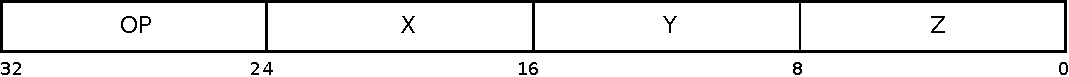
\includegraphics[width=\linewidth]{img/instruction-crop.pdf}

The first byte is the \i{opcode} of the instruction and the other three bytes specify the \i{operands}. Thus, MMIX allows (and uses) 256 instructions with 3 operands, each having 256 possible values. The typical instruction has the meaning "Set register {\tt X} to the result of {\tt Y} OP {\tt Z}". \citep[pg. 2]{mmix-doc}

In this thesis, all instructions are at first outlined with a box that contains the mnemonic, the operands of the instruction and the its effect. Afterwards the instruction is illustrated in further detail -- including special cases and raised \glslink{Exception}{AEs} or \glslink{Exception}{PEs}. The box looks like the following:
\instrtbl
	{\mi{ADD|SUB \$X,\$Y,\$Z|Z}}
	{$\dr{X} \leftarrow s(\dr{Y}) +|- \sdrimm{Z}$}

\noindent This describes the four instructions \mi{ADD}, \mi{ADDI}, \mi{SUB} and \mi{SUBI}. As in this example, many MMIX instructions come in two forms: In the first one, the {\tt Z}-operand is a register, in the second one it is an \glslink{Immediate Value}{immediate value}. Since there is no other difference, these are handled at once by saying "\udrim{Z}". Furthermore, \mi{ADD} and \mi{SUB} are very similar, so that they are grouped together. The notation $s(...)$ denotes, that MMIX interprets it as signed and uses two's complement arithmetic. Otherwise it means that MMIX treats the value as unsigned. Thus, the effect in the box shown above can be read as
\begin{itemize}
	\item \mi{ADD} sets \dr{X} to the result of the addition of \dr{Y} and \dr{Z}, interpreting both as signed values and hence, using signed arithmetic,
	\item \mi{ADDI} sets \dr{X} to the result of the addition of the signed value \dr{Y} and unsigned \glslink{Immediate Value}{immediate value} {\tt Z},
	\item \mi{SUB} sets \dr{X} to the result of the substraction of the signed value \dr{Y} and signed value \dr{Z} and
	\item \mi{SUBI} sets \dr{X} to the result of the substraction of the signed value \dr{Y} and unsigned \glslink{Immediate Value}{immediate value} {\tt Z}.
\end{itemize}
\glslink{Immediate Value}{Immediate values} are always interpreted unsigned in MMIX. Additionally, if one of the operands {\tt X}, {\tt Y} and {\tt Z} is not mentioned in the name, it means implicitly that the corresponding byte has to be zero. If it is not, MMIX will raise a \i{breaks rules} \glslink{Exception}{PE}.

Although the effects description will be straight forward for most of the instructions, it is not meant to be always complete or self-explaining, because that would be too verbose and would require a formal language definition for some instructions. Rather, it should be seen as a quick overview of what the instruction does. Thus, if necessary, the text below the box will clarify the effects description or adds further information.


\section{Registers}

Since the registers are one of the most important entities in MMIX, they are explained at first. MMIX has special, global and local registers, which will be described one after another in this section.

\subsection{Special Registers}

MMIX provides 32 special registers in an array called $sp$ in this thesis\footnote{The special registers may be put in the first 32 slots of the global register array, which is the reason why \sr{G} is always at least 32, as it will be mentioned in the next section. But actually, this is not enforced.}. Most of them will be introduced later as soon as the associated concept or instruction is described. The other ones, that don't fit into a certain category or are very important, are explained here.

\begin{itemize}
	\item \sr{A} - Arithmetic status register:\\
	Since \sr{A} affects many instructions, it is explained first. Its layout is:
	
	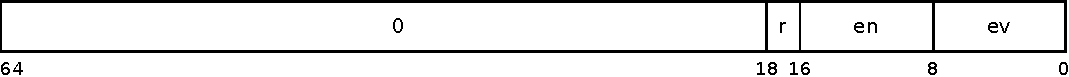
\includegraphics[width=\linewidth]{img/rA-crop.pdf}
	
	The fields $en$ and $ev$ contain \i{enable} and \i{event} bits, both called abbreviated "DVWIOUZX from left to right, where D stands for integer divide check, V for integer overflow, W for float-to-fix overflow, I for invalid operation, O for floating overflow, U for floating underflow, Z for floating division by zero, and X for floating inexact." \citep[pg. 26]{mmix-doc}
	The enable bits control whether an \glslink{Exception}{AE} is raised as soon as the corresponding exceptional condition occurs, while the event bits are set if no \glslink{Exception}{AE} has been raised.
	The field $r$ specifies the rounding mode that is used for floating point numbers, where $00_2$ means round near, $01_2$ round toward zero, $10_2$ round toward $+\infty$ and $11_2$ round toward $-\infty$. All other bits are defined to be zero. \citep[pg. 15 and 26]{mmix-doc}
	
	\item \sr{C} - Cycle counter:\\
	As the name suggests, MMIX increases this special register on every cycle by 1. It can be used to measure the performance of a code snippet, for example. \citep[pg. 32]{mmix-doc}
	\item \sr{I} - Interval counter:\\
	The special register \sr{I} is decreased by 1 on every cycle and causes an \i{interval \glslink{Interrupt}{interrupt}} as soon as it reaches zero. It can also be used for runtime analysis. \citep[pg. 32]{mmix-doc}
	\item \sr{U} - Usage counter:\\
	Register \sr{U} is structured in the following way:
	
	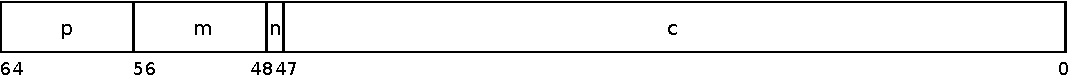
\includegraphics[width=\linewidth]{img/rU-crop.pdf}
	
	The usage count $c$ is increased whenever $OP \& m = p$, where $OP$ is the opcode of an instruction. The bit $n$ indicates whether it should also be done when the \glslink{PC}{instruction pointer} is in the privileged space. \citep[pg. 32]{mmix-doc}
	\item \sr{F} - Failure location register:\\
	This register holds the physical memory address when a parity error or other kinds of memory faults occur. Since an MMIX implementation may use caching, the instruction that caused this error might be long gone before it is detected. \citep[pg. 40]{mmix-doc}
	\item \sr{N} - Serial number:\\
	Register \sr{N} identifies the particular MMIX implementation and is structured as follows:
	
	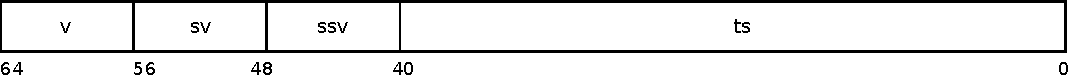
\includegraphics[width=\linewidth]{img/rN-crop.pdf}
	
	The fields $v$, $sv$ and $ssv$ specify the MMIX architecture version. This thesis describes version 1, subversion 0 and subsubversion 0, \ie 1.0.0. The field $ts$ holds the number of seconds from 01/01/1970, 00:00:00 GMT to the date the particular instance of MMIX was built on. \citep[pg. 32]{mmix-doc}
\end{itemize}

\noindent MMIX provides two instructions to read from or write to a special register.

\instrtbl
	{\mi{GET \$X,Z}}
	{\dr{X} $\leftarrow$ \spr{Z}}
\noindent The instruction \mi{GET} sets \dr{X} to the value of special register `Z`. MMIX doesn't keep secrets from the user, \ie all special registers are readable -- even in user mode. \citep[pg. 34]{mmix-doc}

\instrtbl
	{\mi{PUT X,\$Z|Z}}
	{\spr{X} $\leftarrow$ \udrim{Z}}
\noindent \mi{PUT} sets special register `X` to either \dr{Z} or the \glslink{Immediate Value}{immediate value} `Z`. The registers \sr{C}, \sr{N}, \sr{O} and \sr{S} are not writeable in general. \sr{I}, \sr{T}, \sr{TT}, \sr{K}, \sr{Q}, \sr{U} and \sr{V} are writeable in privileged mode only. Additionally, in \sr{A} all bits except \haddrt{3}{FFFF} have to be zero, \sr{G} can't be less than $max(\sr{L},32)$ and not greater than 255. Furthermore, \sr{L} can't be increased with \mi{PUT} and bits in the \i{\glslink{Interrupt}{interrupt} request register} \sr{Q}, that have been set by MMIX since the last execution of \mi{GET \dr{X},\sr{Q}}, can't be unset. In this way, no \glslink{Exception}{PE}, \glslink{Exception}{ME} or \glslink{Interrupt}{interrupt} bit can be lost by accident.\footnote{The restrictions will become more clear as soon as the concepts and instructions working with these registers have been explained.} \citep[pg. 34]{mmix-doc}

\subsection{Global and Local Registers}

MMIX maintains two banks of registers. One for global registers, called $g$, which has at most 256 slots. The other one for local registers, called $l$, which has $2^n$ slots, where $n$ is between 8 and 10. Both can be accessed by the so called \i{dynamic registers}, \dr{0}, \dr{1}, \dots, \dr{255}. MMIX uses the special register \sr{G} to separate them. \sr{G} is always at least 32 at at most 255. When saying \dr{X}, it denotes a global register whenever `X` is greater or equal to \sr{G}. It denotes a local register if it is less than \sr{G}. \citep[pg. 22]{mmix-doc}

Additionally, \sr{L} splits the local registers in two categories. The registers \dr{0}, \dots, \dr{(rL - 1)} are the local registers that are currently in use. The other ones, \dr{(rL)}, \dots, \dr{(rG - 1)}, are called \i{marginal}. If such a register is read, it always yields zero. If \dr{X} is written, where $\sr{L} \le {\tt X} < \sr{G}$, the registers \dr{(rL)}, \dots, \dr{(X - 1)} are set to zero, \dr{X} is set to the desired value and \sr{L} is set to ${\tt X} + 1$. \citep[pg. 22]{mmix-doc}

For example, if \sr{L} is 4 and \sr{G} is 64,
\begin{itemize}
	\item reading \dr{3} would yield the value of $l[3]$,
	\item reading \dr{4} would yield 0,
	\item writing 12 to \dr{5} would set $l[4]$ to 0, $l[5]$ to 12 and \sr{L} to 6,
	\item reading \dr{64} would yield the value of $g[64]$ and
	\item writing 100 to \dr{70} would set $g[70]$ to 100.
\end{itemize}


\section{Integer Arithmetic}

Of course, MMIX provides some instructions to perform integer arithmetic. That is, addition, substraction, multiplication, division and some more. For most of these instructions, MMIX has an unsigned and a signed version. The only difference when adding or substracting is, that the signed versions raise arithmetic \glslink{Exception}{exceptions} -- if necessary -- while the others won't. When multiplying or dividing, the rules for signed or unsigned arithmetic have to be considered.

\subsection{Addition and Substraction}

\instrtbl
	{\mi{ADD|SUB \$X,\$Y,\$Z|Z}}
	{$\dr{X} \leftarrow s(\dr{Y}) +|- \sdrimm{Z}$}
\noindent The sum or difference of \dr{Y} and \udrim{Z} is put into \dr{X}. An integer overflow \glslink{Exception}{AE} is raised if the result is $\ge 2^{63}$ or $< -2^{63}$. \citep[pg. 6]{mmix-doc}

\instrtbl
	{\mi{ADDU|SUBU \$X,\$Y,\$Z|Z}}
	{$\dr{X} \leftarrow (\dr{Y} +|- \udrim{Z}) \bmod 2^{64}$}
\noindent The sum or difference of \dr{Y} and \udrim{Z} is put into \dr{X}. \citep[pg. 6]{mmix-doc}

\instrtbl
	{\mi{NEG \$X,Y,\$Z|Z}}
	{$\dr{X} \leftarrow {\tt Y} - \sdrimm{Z}$}
\noindent MMIX provides a separate instruction for negation to save the programmer from having to put a constant into a register first. This way, \eg \dr{Z} can be negated by saying \mi{NEG \$X,0,\$Z}. It can also be used for building the value $-1$: \mi{NEG \$X,0,1}. The instruction throws an overflow \glslink{Exception}{AE} if the result is $> 2^{63}-1$. \citep[pg. 6]{mmix-doc}

\instrtbl
	{\mi{NEGU \$X,Y,\$Z|Z}}
	{$\dr{X} \leftarrow ({\tt Y} - \udrim{Z}) \bmod 2^{64}$}
\noindent This instruction has the same effect as \mi{NEG}, but does not raise an \glslink{Exception}{AE}. \citep[pg. 6]{mmix-doc}

\subsection{Multiplication and Division}

The more expensive integer arithmetic operations are multiplication and division. MMIX supports 64-bit signed multiplication and division and 128-bit unsigned multiplication and division. The division instructions perform a division and modulo calculation at once. Additionally it is worth noting that MMIX uses the so called \i{floored division}. This means that division rounds towards negative infinity and that the sign of the modulus is always the same as the sign of the divisor \citep[pg. 2]{divmod}. For example, this differs from the x86 architecture, which uses \i{truncated division} \citep[pg. 560]{ia32-sdmv2a}, that rounds towards zero and gives the modulus the sign of the dividend \citep[pg. 2]{divmod}. The following table illustrates the differences:

\begin{table}[h]
	\begin{tabular}{| >{\centering}p{20mm} | >{\centering}p{26mm} | >{\centering}p{26mm} | >{\centering}p{26mm} | >{\centering}p{26mm} |}
		\hline
		\textbf{Y,Z} &
		\textbf{$trunc(Y / Z)$} & \textbf{$trunc(Y \% Z)$} &
		\textbf{$\lfloor Y / Z \rfloor$} & \textbf{$\lfloor Y \% Z \rfloor$}
		\tabularnewline
		\hline
		$+8,+3$ & $+2$ & $+2$ & $+2$ & $+2$
		\tabularnewline
		\hline
		$+8,-3$ & $-2$ & $+2$ & $-3$ & $-1$
		\tabularnewline
		\hline
		$-8,+3$ & $-2$ & $-2$ & $-3$ & $+1$
		\tabularnewline
		\hline
		$-8,-3$ & $+2$ & $-2$ & $+2$ & $-2$
		\tabularnewline
		\hline
	\end{tabular}
	\caption{Comparison of truncated and floored division \citep[pg. 3]{divmod}}
\end{table}
\noindent The differences occur for numbers with different signs only, \ie the unsigned division does behave in the same way regardless of using the floored or truncated algorithm.

\instrtbl
	{\mi{MUL \$X,\$Y,\$Z|Z}}
	{$\dr{X} \leftarrow s(\dr{Y}) * \sdrimm{Z}$}
\noindent The \mi{MUL} instruction sets \dr{X} to the result of the multiplication. It raises an integer overflow \glslink{Exception}{AE} if the result is $\ge 2^{63}$ or $< -2^{63}$. \citep[pg. 14]{mmix-doc}

\instrtbl
	{\mi{MULU \$X,\$Y,\$Z|Z}}
	{$\dr{X} \leftarrow (\dr{Y} * \udrim{Z}) \bmod 2^{64},\quad
	\sr{H} \leftarrow (\dr{Y} * \udrim{Z}) \gg 64$}
\noindent This instruction basically does the same as \mi{MUL}, but treats the operands as unsigned and places the upper 64 bit of the result into the special \i{himult register} \sr{H} and does not raise an overflow \glslink{Exception}{AE}. \citep[pg. 14]{mmix-doc}

\instrtbl
	{\mi{DIV \$X,\$Y,\$Z|Z}}
	{$\dr{X} \leftarrow \lfloor s(\dr{Y})~/~\sdrimm{Z}\rfloor,\quad
	\sr{R} \leftarrow s(\dr{Y}) \bmod \sdrimm{Z}$}
\noindent The instruction \mi{DIV} sets \dr{X} to the result of the division and the \i{remainder register} \sr{R} to the result of the modulo operation. If \sdrim{Z} is zero, a division by zero \glslink{Exception}{AE} is raised, \dr{X} is set to zero and \sr{R} is set to \dr{Y}. An integer overflow \glslink{Exception}{AE} occurs if and only if $-2^{63}$ is divided by $-1$. \citep[pg. 14]{mmix-doc}

\instrtbl
	{\mi{DIVU \$X,\$Y,\$Z|Z}}
	{$\dr{X} \leftarrow \lfloor \sr{D}\dr{Y}~/~\udrim{Z}\rfloor,\quad
	\sr{R} \leftarrow \sr{D}\dr{Y} \bmod \udrim{Z}$}
\noindent Analogous to \mi{MULU}, \mi{DIVU} prefixes the \i{dividend register} \sr{D} to \dr{Y}, resulting in a 128-bit number, and divides it by \udrim{Z}, using unsigned arithmetic. If $\sr{D} \ge \udrim{Z}$ (this includes the case that \udrim{Z} is zero), \dr{X} is set to \sr{D} and \sr{R} is set to \dr{Y}. Additionally, no \glslink{Exception}{AE} is raised. \citep[pg. 14]{mmix-doc}

\medskip

\instrtbl
	{\mi{2ADDU|4ADDU|8ADDU|16ADDU \$X,\$Y,\$Z|Z}}
	{$\dr{X} \leftarrow ((2|4|8|16 * \dr{Y}) + \udrim{Z}) \bmod 2^{64}$}
\noindent As usual, if a number should be divided or multiplied by a power of 2, shifts are much more efficient, which will be described later. MMIX goes even further by providing instructions that multiply a number by 2, 4, 8 or 16 and adding the result to another value. In this way, one can easily e.g. multiply by 3 by saying \mi{2ADDU \$X,\$Y,\$Y}. \citep[pg. 6]{mmix-doc}


\section{Bit Fiddling}

MMIX has quite a few instructions for manipulating bits. At first, the well known bit operations {\tt AND}, {\tt OR}, {\tt NOR}, \dots and shifts are described, because they won't be a surprise.

\subsection{Basic Bit Operations}

\instrtbl
	{\mi{AND|OR|XOR|ANDN|ORN|NAND|NOR|NXOR \$X,\$Y,\$Z|Z}}
	{$\dr{X} \leftarrow \dr{Y} \land|\lor|\oplus|\land \sim|\lor \sim|\mathbin{\overline\land}|\mathbin{\overline\lor}|\mathbin{\overline\oplus} \udrim{Z}$}
\noindent These instructions set \dr{X} to the result of the corresponding bit operation with operands \dr{Y} and \udrim{Z}. The instructions that end with '\mi{N}' logically negate \udrim{Z} first and apply the operation without '\mi{N}' (\mi{OR} or \mi{AND}) afterwards. \citep[pg. 7]{mmix-doc}

\instrtbl
	{\mi{SL|SLU|SR|SRU \$X,\$Y,\$Z|Z}}
	{$\dr{X} \leftarrow \dr{Y} \ll|\ll|\gg|\ggg \udrim{Z}$}
\noindent The instructions for shifting left, \mi{SL} and \mi{SLU}, have the same behaviour, except that \mi{SL} will raise an integer overflow \glslink{Exception}{AE}, if the result is $\ge 2^{63}$ or $< -2^{63}$. \mi{SR} performs an arithmetic right shift, \ie it shifts in copies of the sign bit from the left, and \mi{SRU} performs a logical right shift, \ie it shifts in zeros from the left. Since \udrim{Z} is treaten unsigned, one can't use \mi{SL} to shift right or similar. Additionally it is worth mentioning, that a logical shift left or right of 64 or more will set \dr{X} to zero, whereas an arithmetical shift right of 64 or more will set \dr{X} to $-1$, if \dr{Y} is negative and to zero otherwise. \citep[pg. 10]{mmix-doc}

\subsection{Wyde Operations}

If one liked to put an arbitrary 64-bit constant into a register or manipulate individual wydes of a registers, one could use one of the following 16 instructions.

\instrtbl
	{\mi{SETH|SETMH|SETML|SETL \$X,YZ}}
	{$\dr{X} \leftarrow {\tt YZ} \ll 48|32|16|0$}
\noindent These instructions set the corresponding wyde of \dr{X} to the 16-bit constant {\tt YZ} and all other wydes to zero \citep[pg. 7]{mmix-doc}. That means, for example \mi{SETMH \$X,\haddr{1234}} sets \dr{X} to \haddro{0000}{1234}{0000}{0000}.

\instrtbl
	{\mi{ORH|ORMH|ORML|ORL \$X,YZ}}
	{$\dr{X} \leftarrow \dr{X} \lor ({\tt YZ} \ll 48|32|16|0)$}
\noindent Similarly, these instructions {\tt OR} the 16-bit constant {\tt YZ} into the corresponding wyde of \dr{X} \citep[pg. 7]{mmix-doc}. For example, if \dr{X} is \haddro{0000}{F0F0}{FF00}{0000}, a \mi{ORML \$X,\haddr{0FF0}} will result in \haddro{0000}{F0F0}{FFF0}{0000}.

\instrtbl
	{\mi{ANDNH|ANDNMH|ANDNML|ANDNL \$X,YZ}}
	{$\dr{X} \leftarrow \dr{X}~\land \sim({\tt YZ} \ll 48|32|16|0)$}
\noindent Analogous to the {\tt ORX} family, these instructions remove the bits set in the 16-bit constant {\tt YZ} from the corresponding wyde of \dr{X} \citep[pg. 7]{mmix-doc}. For example, if \dr{X} is \haddro{0000}{F0F0}{FF00}{0000}, a \mi{ANDNML \$X,\haddr{F000}} will result in \haddro{0000}{F0F0}{0F00}{0000}.

\instrtbl
	{\mi{INCH|INCMH|INCML|INCL \$X,YZ}}
	{$\dr{X} \leftarrow (\dr{X} + ({\tt YZ} \ll 48|32|16|0)) \bmod 2^{64}$}
\noindent Last but not least, the {\tt INCX} family adds the 16-bit constant {\tt YZ} to the corresponding wyde of \dr{X}, ignoring overflow \citep[pg. 7]{mmix-doc}. For example, if \dr{X} is \haddro{0000}{F0F0}{FF00}{0000}, an \mi{INCML \$X,\haddr{0101}} will result in \haddro{0000}{F0F1}{0001}{0000} (as shown with the example, other wyde may be affected as well, in contrast to the other wyde instructions).

\subsection{Exotic Bit Operations}

Apart from the simple bit operations just described, MMIX does also support more exotic ones that probably will not be used very often, but allow to do complicated computations in hardware instead of in software, as it would be necessary with other architectures.

\instrtbl
	{\mi{MUX \$X,\$Y,\$Z|Z}}
	{$\dr{X} \leftarrow (\dr{Y} \land \sr{M}) \lor (\udrim{Z} \land \mathbin{\overline{\sr{M}}})$}
\noindent The first rather exotic operation is the \i{bitwise multiplexer} \mi{MUX}. For each bit position $i$, it sets bit $\dr{Y}_i$, if $\sr{M}_i$ is 1, and bit $\udrim{Z_i}$, if $\sr{M}_i$ is 0 \citep[pg. 7]{mmix-doc}. For example, if \sr{M} is \haddro{FFFF}{0000}{FFFF}{0000}, \dr{0} is \haddro{1234}{5678}{90AB}{CDEF} and \dr{1} is \haddro{FFFF}{FFFF}{FFFF}{FFFF}, a \mi{MUX \$X,\$0,\$1} will set \dr{X} to \haddro{1234}{FFFF}{90AB}{FFFF}.

\instrtbl
	{\mi{BDIF|WDIF|TDIF|ODIF \$X,\$Y,\$Z|Z}}
	{$\dr{X}_i \leftarrow max(0,\dr{Y}_i - \udrim{Z_i})$ for each byte|wyde|tetra|octa $i$}
\noindent The second family in this category is the byte, wyde, tetra and octa difference. For example, \mi{BDIF} takes the byte $i$ of \dr{Y}, namely $\dr{Y}_i$, and substracts the byte $\udrim{Z_i}$ from it. If the difference is less than zero, $\dr{X}_i$ is set to zero. Otherwise it is set to the difference. This is done individually for every byte pair. \mi{WDIF}, \mi{TDIF} and \mi{ODIF} behave analogous using wydes, tetras and octas, respectively. These instructions are for example useful, when a graphical application wants to calculate the "pixel difference", \ie the absolute difference of colors, each color component represented as a byte. \citep[pg. 8]{mmix-doc}

\instrtbl
	{\mi{SADD \$X,\$Y,\$Z|Z}}
	{$\dr{X} \leftarrow countbits(\dr{Y} \setminus \udrim{Z})$}
\noindent The \i{sideways addition} \mi{SADD} performs at first the complement of \udrim{Z} and logically ands the result with \dr{Y}. Afterwards the number of set bits in this value is put into \dr{X}. \citep[pg. 9]{mmix-doc} So, for example, if \dr{0} is \haddr{8642} and \dr{1} is \haddr{8002}, a \mi{SADD \$X,\$0,\$1} will put 3 into \dr{X}. Because the difference, \haddr{0640}, has 3 bits set.

\instrtbl
	{\mi{MOR|MXOR \$X,\$Y,\$Z|Z}}
	{$\dr{X} \leftarrow mat(\dr{Y}) \lor|\oplus mat(\udrim{Z})$}
\noindent The last exotic bit operation, called \i{multiple or/exclusive-or}, is the most complicated one. It treats \dr{Y} and \udrim{Z} as $8 \times 8$ bit matrices, using one byte for each column, and performs a kind of matrix product using \mi{OR} or \mi{XOR} instead of the multiplication. More precisely, when the bits of \dr{Y} and \udrim{Z} are numbered as
$$y_{00}y_{01}\ldots y_{07}y_{10}y_{11}\ldots y_{17}\ldots y_{70}y_{71}\ldots y_{77}\quad
z_{00}z_{01}\ldots z_{07}z_{10}z_{11}\ldots z_{17}\ldots z_{70}z_{71}\ldots z_{77},$$
each bit $x_{ij}$ of \dr{X} is set to
$$(y_{0j}\land z_{i0})\lor (y_{1j}\land z_{i1})\lor \cdots \lor (y_{7j}\land z_{i7}).$$
When using \mi{MXOR} instead of \mi{MOR}, the {\tt OR}s are replaced by {\tt XOR}s. \mi{MOR} can be used for example to convert between big endian and little endian. \citep[pg. 9]{mmix-doc} If \dr{0} is \haddro{0123}{4567}{89AB}{CDEF} and \dr{1} is \haddro{0102}{0408}{1020}{4080}, a \mi{MOR \$X,\$0,\$1} will perform the following operation:
\[
\left(%
\begin{array}{*{8}{>{\centering\arraybackslash$}p{1mm}<{$}}}
	0 & 0 & 0 & 0 & 1 & 1 & 1 & 1 \\
	\rowcolor{lightgray}0 & 0 & 1 & 1 & 0 & 0 & 1 & 1 \\
	0 & 1 & 0 & 1 & 0 & 1 & 0 & 1 \\
	0 & 0 & 0 & 0 & 0 & 0 & 0 & 0 \\
	0 & 0 & 0 & 0 & 1 & 1 & 1 & 1 \\
	0 & 0 & 1 & 1 & 0 & 0 & 1 & 1 \\
	0 & 1 & 0 & 1 & 0 & 1 & 0 & 1 \\
	1 & 1 & 1 & 1 & 1 & 1 & 1 & 1
\end{array}
\right)
\lor
\left(%
\begin{array}{*{8}{>{\centering\arraybackslash$}p{1mm}<{$}}}
	0 & 0 & 0 & \cellcolor{lightgray}0 & 0 & 0 & 0 & 1 \\
	0 & 0 & 0 & \cellcolor{lightgray}0 & 0 & 0 & 1 & 0 \\
	0 & 0 & 0 & \cellcolor{lightgray}0 & 0 & 1 & 0 & 0 \\
	0 & 0 & 0 & \cellcolor{lightgray}0 & 1 & 0 & 0 & 0 \\
	0 & 0 & 0 & \cellcolor{lightgray}1 & 0 & 0 & 0 & 0 \\
	0 & 0 & 1 & \cellcolor{lightgray}0 & 0 & 0 & 0 & 0 \\
	0 & 1 & 0 & \cellcolor{lightgray}0 & 0 & 0 & 0 & 0 \\
	1 & 0 & 0 & \cellcolor{lightgray}0 & 0 & 0 & 0 & 0
\end{array}
\right)
=
\left(%
\begin{array}{*{8}{>{\centering\arraybackslash$}p{1mm}<{$}}}
	1 & 1 & 1 & 1 & 0 & 0 & 0 & 0 \\
	1 & 1 & 0 & \cellcolor{lightgray}0 & 1 & 1 & 0 & 0 \\
	1 & 0 & 1 & 0 & 1 & 0 & 1 & 0 \\
	0 & 0 & 0 & 0 & 0 & 0 & 0 & 0 \\
	1 & 1 & 1 & 1 & 0 & 0 & 0 & 0 \\
	1 & 1 & 0 & 0 & 1 & 1 & 0 & 0 \\
	1 & 0 & 1 & 0 & 1 & 0 & 1 & 0 \\
	1 & 1 & 1 & 1 & 1 & 1 & 1 & 1
\end{array}
\right)
\]
Analogous to the matrix product, the highlighted cell in the result matrix is built by {\tt AND}ing each cell in the highlighted row of \dr{Y} with the corresponding highlighted cell of \udrim{Z} individually, starting on the left and top, respectively, and performing an {\tt OR} of all these values. In this case, there is no pair of bits in which both are 1 and thus, the highlighted cell in the result is 0. Doing that for all cells leads to the value \haddro{EFCD}{AB89}{6745}{2301}, \ie the bytes of \dr{0} in the opposite order. \citep[pg. 192]{mmix-buch}


\section{Comparisons}

MMIX has four instructions to compare numbers, which for example can be used for branching. Additionally, it has instructions to conditionally set and zero or set a register.

\instrtbl
	{\mi{CMP \$X,\$Y,\$Z|Z}}
	{$\dr{X} \leftarrow (s(\dr{Y}) > \sdrimm{Z}) - (s(\dr{Y}) < \sdrimm{Z})$}
\noindent The instruction \mi{CMP} compares \dr{Y} with \udrim{Z} using signed arithmetic and puts the result into \dr{X}. If \dr{Y} is less than \udrim{Z}, \dr{X} is set to $-1$, if they are equal, \dr{X} is set to 0 and if \dr{Y} is greater than \udrim{Z}, \dr{X} is set to 1. \citep[pg. 11]{mmix-doc}

\instrtbl
	{\mi{CMPU \$X,\$Y,\$Z|Z}}
	{$\dr{X} \leftarrow (\dr{Y} > \udrim{Z}) - (\dr{Y} < \udrim{Z})$}
\noindent This instruction behaves like \mi{CMPU}, but uses unsigned arithmetic. \citep[pg. 11]{mmix-doc}

\instrtbl
	{\mi{CSN|CSZ|CSP|CSOD|CSNN|CSNZ|CSNP|CSEV \$X,\$Y,\$Z|Z}}
	{if $s(\dr{Y}) <0|=0|>0|odd|\ge0|\ne0|\le0|even$: $\dr{X} \leftarrow \udrim{Z}$}
\noindent The family of conditional set instructions sets \dr{X} to \udrim{Z}, if \dr{Y} is negative, zero, positive, odd, nonnegative, nonzero, nonpositive or even. Otherwise nothing happens. \citep[pg. 11]{mmix-doc}

\instrtbl
	{\mi{ZSN|ZSZ|ZSP|ZSOD|ZSNN|ZSNZ|ZSNP|ZSEV \$X,\$Y,\$Z|Z}}
	{$\dr{X} \leftarrow (s(\dr{Y}) <0|=0|>0|odd|\ge0|\ne0|\le0|even)~?~\udrim{Z}~:~0$}
\noindent Very similar to the conditional set instructions, the zero or set instructions set \dr{X} either to \udrim{Z} or zero, depending on whether \dr{Y} is negative, zero, positive, odd, nonnegative, nonzero, nonpositive or even. \citep[pg. 11]{mmix-doc}

\medskip

MMIX does also provide an atomic \i{compare and swap} instruction. It can be used for interprocess communication with shared memory or to synchronize threads in the same process. Since MMIX is not only designed to work on a single processor, this instruction might also be helpful when independent computers are sharing the same memory. \citep[pg. 25]{mmix-doc}

\instrtblfour
	{\mi{CSWAP \$X,\$Y,\$Z|Z}}
	{if $\vmem{8}{\dr{Y} + \udrim{Z}}~= \sr{P}$:}
	{$\quad \vmem{8}{\dr{Y} + \udrim{Z}}~\leftarrow \dr{X},\quad \dr{X} \leftarrow 1$}
	{else:}
	{$\quad \sr{P} \leftarrow \vmem{8}{\dr{Y} + \udrim{Z}},\quad \dr{X} \leftarrow 0$}
\noindent The \i{compare and swap octabytes} instruction compares \vmem{8}{\dr{Y} + \udrim{Z}} with the special \i{prediction register} \sr{P} and either replaces the octa in memory with \dr{X} or \sr{P} with the octa in memory, depending on whether \sr{P} is equal to the octa. \dr{X} indicates whether the octa in memory has been replaced. \citep[pg. 25]{mmix-doc} For example, one could set \dr{0} to 1, \sr{P} to 0 and do a \mi{CSWAP \$0,\$Y,\$Z|Z}, assuming that $\dr{Y} + \udrim{Z}$ denotes the memory location that is desired for synchronization. If \dr{0} has been set to 1, the lock has been aquired successfully. If not, the whole procedure is repeated. That means, \vmem{8}{\dr{Y} + \udrim{Z}} being 1 or 0 would indicate that someone currently has the lock or not, respectively.


\section{Branches and Jumps}

Of course, MMIX does also need instructions to change the course of computation. To allow programs to use a pipeline implementation of MMIX in an efficient way, it provides both ordinary branches and probable branches. For consistency, the different kinds of comparisons offered by branches are the same as those existing for the conditional set and zero or set instructions.

Similarly to the fact, that the typical "set register {\tt X} to the result of {\tt Y} OP {\tt Z}" instructions come in two versions -- one with {\tt Z} as a register, one with {\tt Z} as an \glslink{Immediate Value}{immediate value} -- the branch and jump instructions also come in two versions. The first one branches or jumps forward, while the second one branches or jumps backwards. The backward versions are suffixed with a '{\tt B}'.

\instrtbl
	{\mi{BN|BZ|BP|BOD|BNN|BNZ|BNP|BEV \$X,@+4*(YZ[-$2^{16}$])}}
	{if $s(\dr{X}) <0|=0|>0|odd|\ge0|\ne0|\le0|even$: $@ \leftarrow @+4*({\tt YZ}[-2^{16}])$}
\noindent If \dr{X} is negative, zero, positive, odd, nonnegative, nonzero, nonpositive or even, the branch will be taken. The forward versions increase the \glslink{PC}{instruction pointer} by $4*{\tt YZ}$, \ie the value of the unsigned 16-bit \glslink{Immediate Value}{immediate value} {\tt YZ} multiplied with the number of bytes of an instruction. The backward versions increase it by $4*({\tt YZ}-2^{16})$. Thus, these instructions allow to change $@$ to any instruction in $(@ - 4*2^{16}) \dots (@ + 4*(2^{16}-1))$. It should be noted, that this category of branches tell MMIX that the branch will probably not be taken. This may affect the runtime on some implementations of MMIX. \citep[pg. 12]{mmix-doc}

\instrtbl
	{\mi{PBN|PBZ|PBP|PBOD|PBNN|PBNZ|PBNP|PBEV \$X,@+4*(YZ[-$2^{16}$])}}
	{if $s(\dr{X}) <0|=0|>0|odd|\ge0|\ne0|\le0|even$: $@ \leftarrow @+4*({\tt YZ}[-2^{16}])$}
\noindent These instructions behave exactly in the same way as the previously introduced ones. The only difference is, that these tell MMIX that the branch will probably be taken. \citep[pg. 12]{mmix-doc}

\instrtbl
	{\mi{JMP @+4*(XYZ[-$2^{24}$])}}
	{$@ \leftarrow @+4*({\tt XYZ}[-2^{24}])$}
\noindent Of course, MMIX has also an instruction to change the \glslink{PC}{instruction pointer} unconditionally: the jump. It simply sets $@$ to $(@+4*({\tt XYZ}[-2^{24}]))$, \ie the forward version increases $@$ by the unsigned 24-bit constant {\tt XYZ}, multiplied by 4. The backward version substracts $2^{24}$ from {\tt XYZ} before multiplying. Thus, one can jump to any instruction in the range $(@ - 4*2^{24}) \dots (@ + 4*(2^{24}-1))$. \citep[pg. 13]{mmix-doc}

\instrtbl
	{\mi{GO \$X,\$Y,\$Z|Z}}
	{$\dr{X} \leftarrow @+4,\quad @ \leftarrow \dr{Y} + \udrim{Z}$}
\noindent To be able to jump to any location in the virtual address space, MMIX has the instruction \mi{GO}. It simply changes the \glslink{PC}{instruction pointer} to $\dr{Y} + \udrim{Z}$. Additionally, \dr{X} is set to the location that ordinary would have been executed next. That allows using \mi{GO} for a simple type of \glslink{Subroutine linkage}{subroutine linkage} by not overwriting \dr{X} in the subroutine and returning via \mi{GO \$X,\$X,0}. But MMIX provides another mechanism, that is much better suited for that task, because it makes subroutines independent of each other, as will be described later in this chapter. An interesting corner case is, that \mi{GO} permits it to jump to addresses that are not tetra-aligned. MMIX will simply set the desired \glslink{PC}{instruction pointer}, but this is not going to be a problem because when loading \vmem{4}{@}, the least significant 2 bits of $@$ are ignored. \citep[pg. 13]{mmix-doc}

\instrtbl
	{\mi{GETA \$X,@+4*(YZ[-$2^{16}$])}}
	{$\dr{X} \leftarrow @+4*({\tt YZ}[-2^{16}])$}
\noindent This instruction does not change the \glslink{PC}{instruction pointer}, but is related because it builds an absolute address from the \glslink{PC}{instruction pointer} and the {\tt YZ} field. \mi{GETA} comes in two versions for forward and backwards calculations and uses the same rules for that as the branches do. \citep[pg. 13]{mmix-doc}


\section{Memory}

The memory hierarchy is one of the more complicated concepts in MMIX. This section starts by explaining the load and store instructions, which are rather simple. Afterwards the structure of the virtual and physical address space is described, followed by the translation mechanism and the translation caches. Finally, the instructions interesting for physical memory caches, which may be present in a particular implementation of MMIX, are introduced.

\subsection{Load Instructions}

MMIX has two kinds of load instructions for each quantity: a signed version and an unsigned version. The difference is that the signed versions treat the number in memory as signed and thus sign-extend the value to 64 bit.

\instrtbl
	{\mi{LDB|LDW|LDT|LDO \$X,\$Y,\$Z|Z}}
	{$\dr{X} \leftarrow s(\vmem{1|2|4|8}{\dr{Y} + \udrim{Z}})$}
\noindent These are the signed load instructions, which set \dr{X} to the byte, wyde, tetra or octa at the specified location in memory. \mi{LDB}, \mi{LDW} and \mi{LDT} will sign-extend the number, \ie the bits in the upper 7, 6 and 4 bytes, respectively, are set to copies of the sign-bit of the number in memory. \citep[pg. 4]{mmix-doc}

\instrtbl
	{\mi{LDBU|LDWU|LDTU|LDOU \$X,\$Y,\$Z|Z}}
	{$\dr{X} \leftarrow $~\vmem{1|2|4|8}{\dr{Y} + \udrim{Z}}}
\noindent As already mentioned, the unsigned versions have the same behaviour, except that they do not sign-extend the values. \mi{LDOU} and \mi{LDO} are completely identical and only exist both for consistency. \citep[pg. 4]{mmix-doc}

\instrtbl
	{\mi{LDHT \$X,\$Y,\$Z|Z}}
	{$\dr{X} \leftarrow~\vmem{4}{\dr{Y} + \udrim{Z}}~\ll 32$}
\noindent The last load instruction, \i{load high tetra}, puts the tetra \vmem{4}{\dr{Y} + \udrim{Z}} into the higher half or \dr{X}. The other half is cleared to zero. \citep[pg. 4]{mmix-doc}

\subsection{Store Instructions}

Analogous to the load instructions, MMIX provides two store instructions for every quantity. In this case, the signed versions throw an integer overflow \glslink{Exception}{AE}, if the number can not be represented with the corresponding quantity, while the unsigned versions do not.

\instrtbl
	{\mi{STB|STW|STT|STO \$X,\$Y,\$Z|Z}}
	{$\vmem{1|2|4|8}{\dr{Y} + \udrim{Z}}~\leftarrow s(\dr{X})$}
\noindent These instructions write the signed number in \dr{X} to the corresponding location in memory. \mi{STB} will throw an integer overflow \glslink{Exception}{AE}, if \dr{X} is not between $-128$ and $+127$, \mi{STW} if \dr{X} is not between $-32,768$ and $+32,767$ and \mi{STT} if \dr{X} is not between $-2,147,483,648$ and $+2,147,483,647$. \mi{STO} will not throw an integer overflow \glslink{Exception}{AE}. \citep[pg. 5]{mmix-doc}

\instrtbl
	{\mi{STBU|STWU|STTU|STOU \$X,\$Y,\$Z|Z}}
	{$\vmem{1|2|4|8}{\dr{Y} + \udrim{Z}}~\leftarrow \dr{X}$}
\noindent The unsigned store instructions are the same as their signed correspondence, but do not test for overflow. \citep[pg. 5]{mmix-doc}

\instrtbl
	{\mi{STHT \$X,\$Y,\$Z|Z}}
	{$\vmem{4}{\dr{Y} + \udrim{Z}}~\leftarrow \dr{X} \gg 32$}
\noindent Similarly to load high tetra, \i{store high tetra} stores the most significant four bytes of \dr{X} to \vmem{4}{\dr{Y} + \udrim{Z}}. \citep[pg. 5]{mmix-doc}

\instrtbl
	{\mi{STCO X,\$Y,\$Z|Z}}
	{$\vmem{8}{\dr{Y} + \udrim{Z}}~\leftarrow {\tt X}$}
\noindent For convenience and efficiency, MMIX provides another store instruction, \i{store constant octabyte}, which stores the unsigned \glslink{Immediate Value}{immediate value} {\tt X} as an octa to the desired location in memory. This saves the programmer from having to put the constant into a register first. \citep[pg. 5]{mmix-doc}

\subsection{Virtual and Physical Address Space}

As already mentioned at the beginning, MMIX has both a 64-bit virtual and physical address space. Their layout is illustrated by the following figure:
\begin{figure}[H]
	\centering
	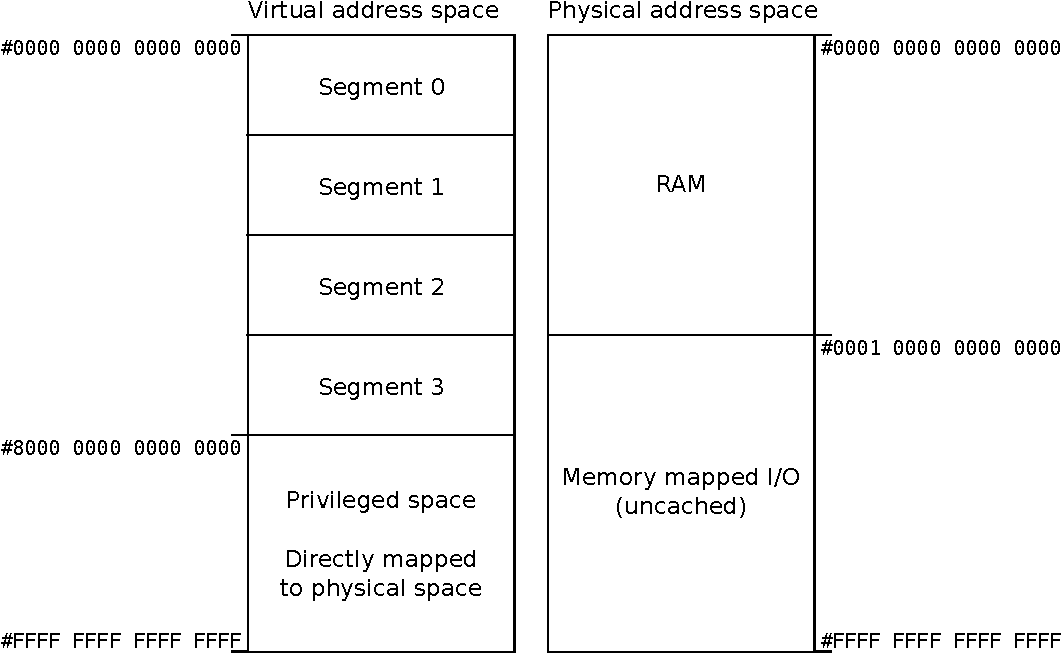
\includegraphics[width=\textwidth]{img/address-spaces-crop.pdf}
	\caption{Virtual and physical address space layout \citep[pg. 35]{mmix-doc}}
\end{figure}
\noindent The virtual address space is divided in user space and privileged space. The privileged space is directly mapped to the physical address space, called m. That means, \vmem{}{{\tt X}}$~=~$m[${\tt X}~\land~$\haddro{7FFF}{FFFF}{FFFF}{FFFF}$]$, if ${\tt X} \ge 2^{63}$. The user space is divided into four segments, determined by the most significant 3 bits using $000_2$, $001_2$, $010_2$ and $011_2$ for segment 0, 1, 2 and 3, respectively. The use of these segments is not restricted by the hardware, but each segment is translated separately, as will be described in the next section.

The first 256 terabyte of the physical space are used for RAM. The remaining space is reserved for I/O devices. The layout of the I/O space is implementation dependent, but MMIX defines that the I/O space is always uncached, regardless of whether the particular MMIX implementation uses caching or not. \citep[pg. 35]{mmix-doc}

\subsubsection{Address Translation}

Besides the privileged space, which is directly mapped to the physical space, the user space is translated to the physical one via a quite complicated scheme. This section describes how this translation works in detail.

\paragraph{The Virtual Translation Register}

The translation is defined by register \sr{V}, which has the following layout:
\begin{figure}[H]
	\centering
	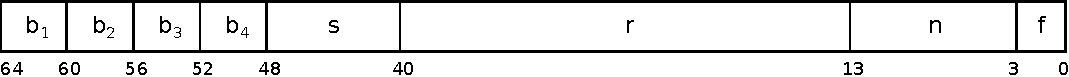
\includegraphics[width=\textwidth]{img/rV-crop.pdf}
\end{figure}
\vspace{-20pt}
\noindent The first two bytes of \sr{V} specify the number of pages in the four segments. Segment $i$ has at most $1024^{b_{i+1}-b_i}$ pages, where $b_0$ is defined to be zero. If $b_i = b_{i+1}$, segment $i$ must have at most one page and if $b_i > b_{i+1}$, segment i must be empty. For example,
\begin{itemize}
	\item if $b_1 = 1$, $b_2 = 2$, $b_3 = 3$ and $b_4 = 4$, all segments have at most 1024 pages,
	\item if $b_1 = 3$, $b_2 = 2$, $b_3 = 1$ and $b_4 = 0$, segment 0 has at most $1024^3$ pages and all other segments are empty and
	\item if $b_1 = 1$, $b_2 = 0$, $b_3 = 0$ and $b_4 = 0$, segment 0 has at most 1024 pages, segment 1 is empty and segments 2 and 3 have both at most 1 page.
\end{itemize}
The next field, called $s$, specifies that the page size is $2^s$, where $s$ has to be at least 13 and at most 48. The field $r$ tells MMIX the \i{root location}, which will be described in further detail shortly. The field $n$ holds the \i{address space number} and last but not least, $f$ is the \i{function field}, which specifies whether virtual address translation will be done by software ($f=1$) or by hardware ($f=0$). Other values are illegal. If translation by software is requested, MMIX ignores $b_1$, $b_2$, $b_3$, $b_4$ and $r$ of \sr{V} and lets the software decide how the actual translation mechanism works. That means, the following structures and concepts only apply if hardware translation is used. \citep[pg. 36]{mmix-doc}

\paragraph{The Root Location}

The field $r$ specifies an area in memory that holds the \glslink{Paging}{paging} structures for the current virtual address space. For each segment $i$ it holds $b_{i+1} - b_i$ page tables with either \i{page table entries} (PTEs) or \i{page table pointers} (PTPs), which are described in the next paragraphs. The page tables in the root location are, one could say, the "first layer" of the translation, because PTPs point to other page tables that reside in a different location in memory.

\paragraph{Page Table Entries}

A PTE defines to which page in physical memory a page in virtual memory is mapped to. Additionally it specifies the access permissions for that page. A PTE looks like the following:
\begin{figure}[H]
	\centering
	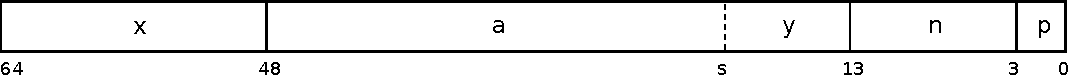
\includegraphics[width=\textwidth]{img/PTE-crop.pdf}
\end{figure}
\vspace{-20pt}
\noindent The field $a$ holds the physical address divided by the page size, \ie the physical address is $a * 2^s$. The field $n$ is the address space number, which has to be equal to $n$ in \sr{V}. The access permissions are defined by $p$ with bit 0 for executing, bit 1 for writing and bit 2 for reading. That means, for example $p=101_2$ makes the page readable and executable. The fields $x$ and $y$ are ignored by the hardware, which allows the operating system to use them for any purpose. \citep[pg. 36]{mmix-doc} It is noteworthy, that $y$ would be empty, if the page size were $2^{13}$, and $a$ would be empty, if the page size were $2^{48}$. Additionally, the layout of a PTE clarifies the reason for the page size restrictions.

\paragraph{Page Table Pointers}

PTPs are pointers to other page tables that may either hold PTPs as well or hold PTEs. They have the following layout:
\begin{figure}[H]
	\centering
	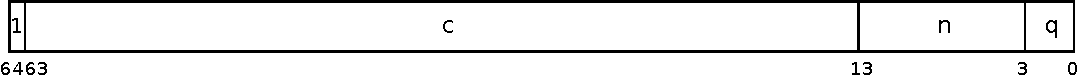
\includegraphics[width=\textwidth]{img/PTP-crop.pdf}
\end{figure}
\vspace{-20pt}
\noindent Similarly to the field $a$ of a PTE, the field $c$ of a PTP specifies the address of the page table this PTP links to, divided by the page size. The field $n$ has to match $n$ in \sr{V} as well, while $q$ is ignored and the most significant bit has to be 1. This forces the operating system to put a privileged address into a PTP, which is -- as already mentioned -- directly mapped. \citep[pg. 36]{mmix-doc}

\paragraph{The Translation Process}

Finally, the actual translation process should be described. If address $A$ should be translated, the segment is determined by $i = \lfloor A / 2^{61} \rfloor$. The page number in this segment is $A_p = \lfloor (A~\land~$\haddro{1FFF}{FFFF}{FFFF}{FFFF}$) / 2^s \rfloor$. Assuming that $A_p$ is equal to $(a_4a_3a_2a_1a_0)_{1024}$ (in the number system with base 1024), the translation works as follows:
\begin{itemize}
	\item if $a_4=a_3=a_2=a_1=0$, the PTE $e$ is \pmem{8}{2^{13}(r + b_i) + 8a_0} and thus, \vmem{}{A} corresponds to \pmem{}{2^s*e.a + (A \bmod 2^s)}.
	\item if $a_4=a_3=a_2=0$, the auxiliary PTP $p$ is used first, \ie \pmem{8}{2^{13}(r + b_i + 1)+8a_1}. In this case, the PTE is \pmem{8}{2^{13}*p.c + 8a_0}. Thus, one level of indirection is used.
	\item if $a_4=a_3=0$, two levels of indirection are used. That means, the first PTP $p1$ is \pmem{8}{2^{13}(r + b_i + 2)+8a_2} and determines the next PTP. This one, $p2$, is \pmem{8}{2^{13}*p1.c + 8a_1}. And finally the PTE is \pmem{8}{2^{13}*p2.c + 8a_0}.
	\item \dots
\end{itemize}
\citep[pg. 36]{mmix-doc} It is noteworthy, that when using the minimum page size of $2^{13}$, four levels of indirection are sufficient to cover a whole segment. Because $2^{13} * 1024 * 1024^4 = 2^{63}$ covers even more than one segment. Additionally, it is worth mentioning that the first slot in PTP page tables in the root location is actually never used. Because this slot is covered by the previous page table in the root location.

\paragraph{Example}

To clarify the just explained concepts and to show the layout in memory, which they imply, the following goes through an example. Supposed that \sr{V} and the \glslink{Paging}{paging} structures in memory are filled as:
\begin{figure}[H]
	\centering
	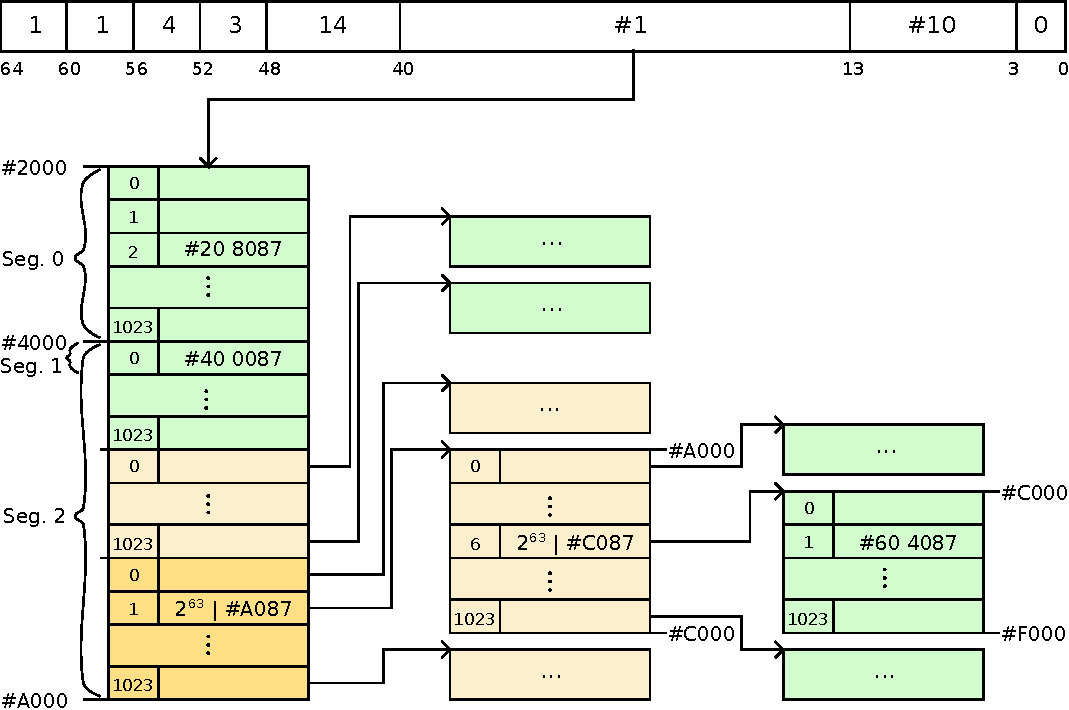
\includegraphics[width=\textwidth]{img/paging-example-crop.pdf}
	\caption{Paging example}
\end{figure}
\noindent Hence, segment 0 has 1024 pages, segment 1 has only one page, segment 2 has $1024^3$ pages and segment 3 has no pages at all. Additionally, the page size is $2^{14}$, the address space number is \haddr{10} and the root location is \haddr{2000} (\haddr{1}$~\ll 13$). The root location is displayed on the left, while auxiliary page tables are on the right. Furthermore, the green cells contain PTEs, the light orange cells PTPs of level 1 and the orange cells PTPs of level 2. For demonstration purposes, the cells display the page table index on the left and some show the content as an octa on the right. All PTEs and PTPs end with \haddr{87}, because they have to match the $n$ of \sr{V} and have read, write and execute permissions (which actually has no special reason here).

Ignoring the special case that segment 1 and 2 overlap for a while, one can see that the number of page tables in the root location for segment $i$ corresponds to $b_{i+1} - b_i$. The first page table does always contain PTEs, the second one PTPs of level 1 and so on. Each page table has 1024 slots and therefore it is 8192 bytes large. As the arrows show, PTPs do always point to another page table.

Since in this case $b_1$ is equal to $b_2$, segment 1 has only one page. An additional consequence of the interpretation of the segment sizes and the translation mechanism is, that -- as the figure shows -- the page in segment 1 is mapped by the first PTE of the page table responsible for segment 2. Thus, this PTE is used for the first page both in segment 1 and segment 2.

% TODO let's
To demonstrate the translation process, let's go through a few examples:
\begin{itemize}
	\item \haddr{80FF}:\\
	Obviously, \haddr{80FF} belongs to segment 0 and the page number is $(00002)_{1024}$. As described, in this case the PTE is \pmem{8}{2^{13}($\lstinline`\#1`$+0) + 8*2}$~=~$\pmemh{8}{2010}. The third slot of the first page table in segment 0 contains \haddrt{20}{8087}, which means that the physical base address for that page is \haddrt{20}{8000} and thus, the resulting physical address \haddrt{20}{80FF}.
	\item \haddro{2000}{0000}{0000}{1234}:\\
	This address belongs to segment 1 and has the page number $(00001)_{1024}$. The PTE is \pmem{8}{2^{13}($\lstinline`\#1`$+1) + 8*0}$~=~$\pmem{8}{$\lstinline`\#4000`$}$~=~$\haddrt{40}{0087}. Hence, the resulting physical address is \haddrt{40}{1234}.
	\item \haddro{4000}{0004}{0600}{4000}:\\
	Last but not least, this address belongs to segment 2 and has the page number $(00161)_{1024}$. Thus, the level 2 PTP is \pmem{8}{2^{13}($\lstinline`\#1`$+3) + 8*1}$~=~$\pmemh{8}{8008}, which loads \haddro{8000}{0000}{0000}{A087}. Therefore it links to the PTE \pmem{8}{$\lstinline`\#A000`$ + 8*6}$~=~$\pmemh{8}{A030}, which in turn is \haddro{8000}{0000}{0000}{C087}. The last step loads the PTE \pmem{8}{$\lstinline`\#C000`$ + 8*1} $=~$\pmemh{8}{C008}$~=~$\haddrt{60}{4087}, so that the final address is \haddrt{60}{4000}.
\end{itemize}

\subsubsection{Translation Caches}

To prevent that every memory access requires this lengthy translation from virtual to physical addresses, MMIX uses a \i{translation cache}. This is also known as \i{translation lookaside buffer} (TLB). However, MMIX calls it translation cache or short TC. The exact behaviour or whether separate caches for instructions and data exist, is not enforced by the architecture. But MMIX defines that the TC contains \i{translation keys}, which are associated with \i{translations}. The translation key is basically the virtual address, whereas the translation is more or less the physical address. The key is structured as follows:
\begin{figure}[H]
	\centering
	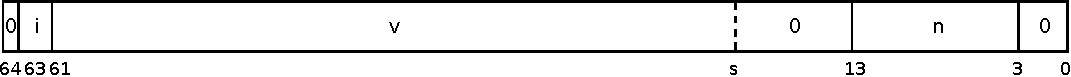
\includegraphics[width=\textwidth]{img/TC-key-crop.pdf}
\end{figure}
\vspace{-20pt}
\noindent As usual, the field $n$ holds the address space number. The field $i$ is the segment number and $v$ is the virtual address, divided by the page size. The other parts are defined to be zero. The layout of a translation is:
\begin{figure}[H]
	\centering
	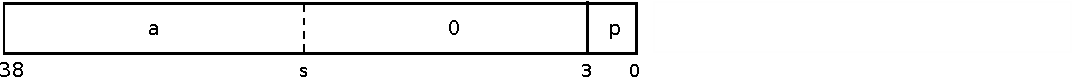
\includegraphics[width=\textwidth]{img/TC-trans-crop.pdf}
\end{figure}
\vspace{-20pt}
\noindent Similarly to a PTE, the field $a$ holds the physical address, divided by the page size. The last three bits contain the protection bits, whereas the other bits are defined to be zero. \citep[pg. 37]{mmix-doc}

Of course, the operating system needs a way to keep the TC up to date, when for example removing PTEs or changing their protection bits. Therefore, MMIX provides the instruction \mi{LDVTS}.

\instrtbl
	{\mi{LDVTS \$X,\$Y,\$Z|Z}}
	{$\dr{X} \leftarrow updateTC(\dr{Y} + \udrim{Z})$}
\noindent The instruction \i{load virtual translation status} updates the translation cache for $\dr{Y} + \udrim{Z}$, which should have the form of a translation key, except that the least significant three bits need not be zero. \dr{X} will be set to 0 if the key is not in the TC, 1 if it is present for instructions, 2 if it is present for data and 3 if it is present for both. If this key is present in the TC, the protection bits will be replaced with $(\dr{Y} + \udrim{Z})~\land~$\haddr{7}. If these are zero, the key will be removed. \citep[pg. 37]{mmix-doc}

\subsubsection{Physical Memory Caches}

As already mentioned, a particular implementation of MMIX may use caches for the RAM space of the physical memory. Which caches are present and how they are organized, is completely implementation dependent. But MMIX provides several instructions to allow a more efficient use of the caches and to keep them up to date. Similarly to the translation caches, MMIX has in mind that an implementation may provide separate caches for instructions and data.

\instrtbl
	{\mi{LDUNC \$X,\$Y,\$Z|Z}}
	{$\dr{X} \leftarrow s(\vmem{8}{\dr{Y} + \udrim{Z}})$}
\noindent The first instruction in this category is \mi{LDUNC}, \i{load octa uncached}. It has  the same behaviour as \mi{LDO}, but tells MMIX "that the loaded octabyte (and its neighbors in a cache block) will probably not be read or written in the near future" \citep[pg. 24]{mmix-doc}.

\instrtbl
	{\mi{STUNC \$X,\$Y,\$Z|Z}}
	{$\vmem{8}{\dr{Y} + \udrim{Z}}~\leftarrow s(\dr{X})$}
\noindent The instruction \i{store octa uncached} has the same meaning as \mi{STO} and tells MMIX the same as \mi{LDUNC} does. \citep[pg. 24]{mmix-doc}

\instrtbl
	{\mi{PRELD|PREGO|PREST X,\$Y,\$Z|Z}}
	{-}
\noindent These instructions have no (visible) effect, but inform MMIX that the ${\tt X}+1$ bytes \vmem{1}{\dr{Y} + \udrim{Z}}, \dots, \vmem{1}{\dr{Y} + \udrim{Z} + {\tt X}} will probably be loaded/stored, used as instructions or stored before loaded for \mi{PRELD}, \mi{PREGO} or \mi{PREST}, respectively. That means, if \mi{PRELD} is used, it might make sense to load these bytes into the data cache. If \mi{PREGO} is used, MMIX might put these bytes into the instruction cache and if \mi{PREST} is used, MMIX may ignore the current bytes in memory. Therefore, if these bytes are requested and are not yet in cache, MMIX does not need to load them from memory, because they will be written before they are read anyway. MMIX does also define, that no protection fault occurs for these instructions. \citep[pg. 24]{mmix-doc}

\instrtbltwo
	{\mi{SYNCD X,\$Y,\$Z|Z}}
	{$caches[\dr{Y} + \udrim{Z}:{\tt X}+1] \rightarrow$~\pmem{}{\dr{Y} + \udrim{Z}:{\tt X}+1}}
	{if in privileged mode: $caches[\dr{Y} + \udrim{Z}:{\tt X}+1] \leftarrow \varnothing$}
\noindent The instruction \i{synchronize data} forces the hardware to make sure that all data for the ${\tt X}+1$ bytes \vmem{1}{\dr{Y} + \udrim{Z}}, \dots, \vmem{1}{\dr{Y} + \udrim{Z} + {\tt X}} is present in memory (and not only in cache). If executed in the privileged space, it does additionally force MMIX to remove these bytes from the data cache. Again, no protection fault will occur if the memory is not accessible. \citep[pg. 24]{mmix-doc}

\instrtblfour
	{\mi{SYNCID X,\$Y,\$Z|Z}}
	{if in user mode:}
	{$\quad IC[\dr{Y} + \udrim{Z}:{\tt X}+1] \leftrightarrow DC[\dr{Y} + \udrim{Z}:{\tt X}+1]$}
	{else:}
	{$\quad caches[\dr{Y} + \udrim{Z}:{\tt X}+1] \leftarrow \varnothing$}
\noindent When executed in user space, \i{synchronize instructions and data} forces the hardware to make sure that the ${\tt X}+1$ bytes \vmem{1}{\dr{Y} + \udrim{Z}}, \dots, \vmem{1}{\dr{Y} + \udrim{Z} + {\tt X}} will be interpreted correctly when used as instructions. That means, MMIX should synchronize its data cache with its instruction cache (\eg because instructions might have been manually fabricated and might thus only be present in the data cache yet). When \mi{SYNCID} is executed in privileged space, the hardware has to remove these bytes from all caches \i{without} writing it to memory. As with \mi{SYNCD}, no protection faults can occur. \citep[pg. 24,25]{mmix-doc}

\instrtbleight
	{\mi{SYNC XYZ}}
	{if ${\tt XYZ} = 0$: drain pipeline}
	{if ${\tt XYZ} = 1$: drain stores}
	{if ${\tt XYZ} = 2$: drain loads}
	{if ${\tt XYZ} = 3$: drain loads and stores}
	{if ${\tt XYZ} = 4$: go into power-saver mode}
	{if ${\tt XYZ} = 5$: flush caches to memory}
	{if ${\tt XYZ} = 6$: clear TCs}
	{if ${\tt XYZ} = 7$: clear caches}
\noindent The last instruction in this category is \i{synchronize}, which is used for various purposes, whereas the 24-bit constant {\tt XYZ} determines what action is performed. The first four actions drain the pipeline, in the sense that it stalls until all preceding instructions are finished (or all stores, loads, loads and stores for 1, 2, 3, respectively, are finished before the corresponding instructions after them). The fifth action tells MMIX to go into a power-saver mode, \ie MMIX is allowed to execute instructions slower or not at all until some kind of signal arrives. The next one writes all cache content to main memory, while the last two simply remove all entries from the TCs or the instruction and data caches. Using \mi{SYNC} with ${\tt XYZ} > 3$ is allowed in privileged mode only. \citep[pg. 25]{mmix-doc}


\section{Floating Point Operations}

Besides integer arithmetic, MMIX does also provide instructions to work with floating point numbers. The floating point arithmetic respects the IEEE/ANSI Standard 754. Since 64-bit quantities are the words of MMIX, arithmetic does always work with 64-bit floats, \ie "doubles". But MMIX does also support some instructions to convert from 64-bit floats to 32-bit floats and the other way around.

\subsection{Representation of Floating Point Numbers}

A 64-bit floating point number has the following structure:
\begin{figure}[H]
	\centering
	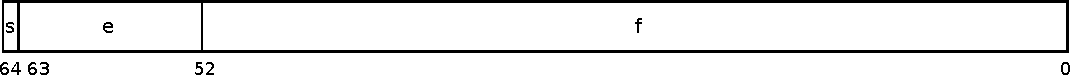
\includegraphics[width=\textwidth]{img/float-crop.pdf}
\end{figure}
\vspace{-20pt}
\noindent That means, it has a sign-bit $s$, an 11-bit exponent $e$ and a 52-bit fraction $f$. Taking $e$ as an unsigned integer and $f$ as a fraction between 0 and $(.111\dots1)_2 = 1 - 2^{-52}$, an octabyte has the following significance:
$$\vbox{\halign{\hfil$\pm#$,\quad if &#\hfil\cr
	0.0								& $e = f = 0$ (zero);\cr
	2^{\mkern1mu e - 1023}(1 + f)	& $0 < e < 2047$ (normal);\cr
	2^{-1022}f						& $e = 0$ and $f > 0$ (subnormal);\cr
	\infty							& $e = 2047$ and $f = 0$ (infinite);\cr
	\NaN(f)							& $e = 2047$ and $0 < f < 1/2$ (signaling NaN);\cr
	\NaN(f)							& $e = 2047$ and $f \ge 1/2$ (quiet NaN).\cr
}}$$
As shown, there are two representations for zero - a positive and a negative one. There are \i{normal} numbers, that can range from approximately $\pm 10^{-308}$ to $\pm 10^{308}$. Additionally \i{subnormal} numbers (also called \i{denormal} or \i{denormalized} numbers) are supported, which can range from approximately $\pm 10^{-324}$ to $\pm 10^{-308}$, but have fewer bits of precision. If the exponent has the maximum value, \ie 2047, it encodes infinity or \i{not a number} (\NaN). The latter distinguishes between \i{signaling} and \i{quiet} \NaN. Signaling \NaNs raise an invalid \glslink{Exception}{AE} when they are used, while quiet \NaNs won't. \citep[pg. 15]{mmix-doc}

Furthermore, the standard defines that four rounding modes should be available: round to nearest (and to even in case of ties, \ie the least significant bit should be zero), round off (toward zero), round up (toward $+\infty$) and round down (toward $-\infty$). MMIX uses the special register \sr{A} to specify the rounding mode. Additionally, all instructions having only one operand, specify the rounding mode with operand {\tt Y} using ${\tt Y}=0$ for the round mode in \sr{A}, ${\tt Y}=1$ for round off, ${\tt Y}=2$ for round up, ${\tt Y}=3$ for round down and ${\tt Y}=4$ for round near. \citep[pg. 15 and 21]{mmix-doc}

Last but not least, there are five kinds of \glslink{Exception}{arithmetic exceptions}, that can occur when working with floating point numbers:
\begin{enumerate}
	\item Floating overflow (value too large to be representable),
	\item Floating underflow (value too small to be representable),
	\item Floating divide by zero,
	\item Floating inexact (exact result not representable) and
	\item Floating invalid (square root of negative number, using signaling \NaN, \dots).
\end{enumerate}
As already said, all of these will either raise an \glslink{Exception}{AE} or set the corresponding \i{event bit} in \sr{A}, depending on whether the corresponding \i{enable bit} in \sr{A} is set or not. \citep[pg. 15]{mmix-doc}

\subsection{Arithmetic}

The first category of floating point operations are the arithmetic instructions. The floating point instructions don't have an \glslink{Immediate Value}{immediate} version, because it doesn't make much sense to specify a float with a single byte. Additionally, this section uses $f(\dots)$ to indicate that a value is interpreted as a 64-bit floating point number.

\instrtbl
	{\mi{FADD|FSUB \$X,\$Y,\$Z}}
	{$\dr{X} \leftarrow f(\dr{Y}) +|- f(\dr{Z})$}
\noindent \mi{FADD} computes the sum of \dr{Y} and \dr{Z}, treating them as floating point numbers and puts the result in \dr{X}. \mi{FSUB} performs the same operation, but switches the sign of \dr{Z} first, if \dr{Z} is not \NaN. If the sum of $(+\infty)+(-\infty)$ or $(-\infty)+(+\infty)$ is computed, an invalid \glslink{Exception}{AE} will be raised. \citep[pg. 16]{mmix-doc}

\instrtbl
	{\mi{FMUL|FDIV \$X,\$Y,\$Z}}
	{$\dr{X} \leftarrow f(\dr{Y}) *|/ f(\dr{Z})$}
\noindent These instructions multiply or divide the floating point numbers \dr{Y} and \dr{Z}. Several cases result in an invalid \glslink{Exception}{AE}, like $(\pm 0.0)*(\pm \infty)$, $(\pm 0.0)/(\pm 0.0)$ or $(\pm \infty)/(\pm \infty)$. Of course, dividing by $(\pm 0.0)$ raises a floating divide by zero \glslink{Exception}{AE}. \citep[pg. 16]{mmix-doc}

\instrtbl
	{\mi{FREM \$X,\$Y,\$Z}}
	{$\dr{X} \leftarrow f(\dr{Y}) \bmod f(\dr{Z})$}
\noindent The \i{floating remainder} instruction computes the remainder and puts it into \dr{X}. This is defined "to be $\dr{Y} - n * \dr{Z}$, where $n$ is the nearest integer to $\dr{Y}/\dr{Z}$, and $n$ is an even integer in case of ties" \citep[pg. 16]{mmix-doc}. If \dr{Y} is infinite and/or \dr{Z} is zero, an invalid \glslink{Exception}{AE} will be raised. \citep[pg. 16]{mmix-doc}

\instrtbl
	{\mi{FSQRT \$X,Y,\$Z}}
	{$\dr{X} \leftarrow \sqrt{f(\dr{Z})},\quad$ using round-mode {\tt Y}}
\noindent The last one in this family is \i{floating square root}. It puts the square root of \dr{Z} into \dr{X}. An invalid \glslink{Exception}{AE} is raised will be \dr{Z} is negative, except for $-0.0$. \citep[pg. 17]{mmix-doc}

\subsection{Comparison}

Of course, besides doing arithmetic, one has to be able to compare floating point numbers. This does not work well using the integer comparison instructions, because one would have to take care of negative numbers, $+0.0$, $-0.0$ and \NaN manually. Therefore, the floating point comparisons simplify that task.

\instrtbl
	{\mi{FCMP \$X,\$Y,\$Z}}
	{$\dr{X} \leftarrow (f(\dr{Y}) > f(\dr{Z})) - (f(\dr{Y}) < f(\dr{Z}))$}
\noindent As the effect description shows, \mi{FCMP} is basically the same as \mi{CMP}, but treats the operands as floating point numbers. Thus, \dr{X} will be set to $-1$, if \dr{Y} is less than \dr{Z}, 0 if \dr{Y} is equal to \dr{Z} and 1 if \dr{Y} is greater than \dr{Z}. It will raise an invalid \glslink{Exception}{AE} and set \dr{X} to zero, if \dr{Y} or \dr{Z} is \NaN. \citep[pg. 17]{mmix-doc}

\instrtbl
	{\mi{FEQL \$X,\$Y,\$Z}}
	{$\dr{X} \leftarrow (f(\dr{Y}) = f(\dr{Z}))~?~1~:~0$}
\noindent \i{Floating equal to} sets \dr{X} to 1, if \dr{Y} and \dr{Z} are equal. But it is noteworthy, that \NaN is not equal to anything and $-0.0$ is equal to $+0.0$. \citep[pg. 17]{mmix-doc}

\instrtbl
	{\mi{FUN \$X,\$Y,\$Z}}
	{$\dr{X} \leftarrow (f(\dr{Y}) = \NaN \lor f(\dr{Z}) = \NaN)~?~1~:~0$}
\noindent The last comparison instruction is \i{floating unordered} and sets \dr{X} to 1, if \dr{Y} and \dr{Z} are considered \i{unordered}, \ie at least one of them is \NaN. \citep[pg. 17]{mmix-doc}

\subsection{Neighborhood Comparison}

Because of the limited precision of floating point numbers, operations might produce inexact results. The larger the numbers, the larger the potential difference of the produced result to the exact result. For that reason, an absolute comparison of floats, as the last section described, is not always desired. Therefore, MMIX offers another category of instructions that allow comparisons with respect to an \i{epsilon} and depending on the magnitude of the floating point numbers in question.

At first, MMIX defines a so called \i{neighborhood} of a number. Assuming that epsilon is a float called $\epsilon$, the float $u$ with fraction $f$ and exponent $e$ has the neighborhood:
\[
	N_\epsilon(u) = \left\{
	\begin{array}{l l}
		\{x \mid |x-u| \le 2^{e-1022}\epsilon\}
			& \quad \text{if $u$ is normal}\\
		\{x \mid |x-u| \le 2^{-1021}\epsilon\}
			& \quad \text{if $u$ is subnormal}\\
		\{0\}
			& \quad \text{if $u$ is zero}\\
		\{\pm \infty\}
			& \quad \text{if $u$ is $\pm \infty$ and $\epsilon < 1$}\\
		\{\text{everything except $\mp \infty$}\}
			& \quad \text{if $u$ is $\pm \infty$ and $1 \le \epsilon < 2$ and}\\
		\{\text{everything}\}
			& \quad \text{if $u$ is $\pm \infty$ and $\epsilon \ge 2$.}\\
	\end{array} \right.
\]
\citep[pg. 19]{mmix-doc} Without going into the details of this definition, it basically means that the neighborhood of a normal float depends on its exponent. That is, the larger the exponent, the larger the neighborhood.

Displayed graphically (and a bit exaggerated for demonstration purposes), the neighborhoods of a few numbers might look like the following:
\begin{figure}[H]
	\centering
	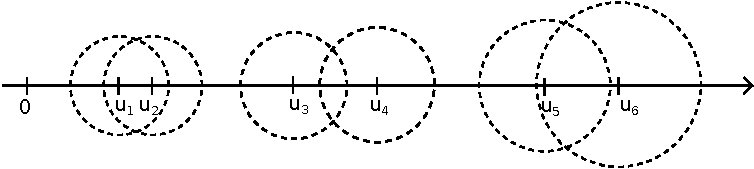
\includegraphics[width=\textwidth]{img/cmpe-less-crop.pdf}
	\caption{Example neighborhoods, demonstrating float relationships}
\end{figure}
\noindent MMIX distinguishes four cases when comparing floats $u$ and $v$ with respect to $\epsilon$:
\begin{enumerate}
	\item $u \approx v$, if $u \in N_\epsilon(v)$ and $v \in N_\epsilon(u)$.\\
	That means, two numbers will be considered \i{equivalent}, if both are in the neighborhood of the corresponding other number. In the example, only $u_1 \approx u_2$, because $u_1 \in N_\epsilon(u_2)$ and $u_2 \in N_\epsilon(u_1)$.
	\item $u \sim v$, if $u \in N_\epsilon(v)$ or $v \in N_\epsilon(u)$.\\
	Thus, two numbers will be considered \i{similar}, if only one of them belongs to the neighborhood of the corresponding other number. For example, $u_5 \sim u_6$, because $u_5 \in N_\epsilon(u_6)$, but $u_6 \notin N_\epsilon(u_5)$.
	\item $u \prec v$, if $u < N_\epsilon(v)$ and $N_\epsilon(u) < v$.\\
	For example, $u_3 \prec u_4$ because $u_3$ is less than all numbers in $N_\epsilon(u_4)$ and all numbers in $N_\epsilon(u_3)$ are less than $u_4$.
	\item $u \succ v$, if $u > N_\epsilon(v)$ and $N_\epsilon(u) > v$.\\
	Analogous, $u_4 \succ u_3$.
\end{enumerate}
\citep[pg. 19]{mmix-doc} The following instructions are based on this definition and use the special \i{epsilon register} \sr{E} for $\epsilon$.

\instrtbl
	{\mi{FCMPE \$X,\$Y,\$Z}}
	{$\dr{X} \leftarrow (f(\dr{Y}) \succ f(\dr{Z})~(\sr{E})) - (f(\dr{Y}) \prec f(\dr{Z})~(\sr{E}))$}
\noindent Analogous to \mi{FCMP}, \mi{FCMPE} - called \i{floating compare with respect to epsilon} - compares \dr{Y} with \dr{Z} according to the definition above and sets \dr{X} to $-1$, 0 or 1. It should be noted, that \dr{X} will be set to zero, if \dr{Y} is similar \i{or} equivalent to \dr{Z}. An invalid \glslink{Exception}{AE} will be raised, if \dr{Y}, \dr{Z} or \sr{E} is \NaN or \sr{E} is negative. \citep[pg. 19]{mmix-doc}

\instrtbl
	{\mi{FEQLE \$X,\$Y,\$Z}}
	{$\dr{X} \leftarrow (f(\dr{Y}) \approx f(\dr{Z})~(\sr{E}))~?~1~:~0$}
\noindent Similarly to \mi{FEQL}, \mi{FEQLE} will set \dr{X} to 1, if \dr{Y} is equivalent to \dr{Z}, depending on \sr{E}. It raises the same \glslink{Exception}{arithmetic exceptions} as \mi{FCMPE}. \citep[pg. 19]{mmix-doc}

\instrtbl
	{\mi{FUNE \$X,\$Y,\$Z}}
	{$\dr{X} \leftarrow (f(\dr{Y}) = \NaN \lor f(\dr{Z}) = \NaN \lor \sr{E} = \NaN \lor \sr{E} < 0)~?~1~:~0$}
\noindent The last one in this group is \mi{FUNE}, which will set \dr{X} to 1, if \dr{Y}, \dr{Z} or \sr{E} are exceptional as described for \mi{FCMPE} and \mi{FEQLE}. \citep[pg. 19]{mmix-doc}

\subsection{Conversion between Float and Integer}

MMIX offers three groups of instructions to convert an integer to a floating point number and the other way around.

\instrtbl
	{\mi{FIX|FIXU \$X,Y,\$Z}}
	{$\dr{X} \leftarrow (int)f(\dr{Z}) \bmod 2^{64},\quad$ using round-mode {\tt Y}}
\noindent The instructions \i{convert floating to fixed} and \i{convert floating to fixed unsigned} take \dr{Z} as a float, convert it to an integer and put it into \dr{X}. Only when using \mi{FIX}, an invalid \glslink{Exception}{AE} will be raised if \dr{Z} is infinite or \NaN and a float-to-fix \glslink{Exception}{AE} will occur, if the result is less than $-2^{63}$ or greater than $2^{63}-1$. \citep[pg. 20]{mmix-doc}

\instrtbl
	{\mi{FINT \$X,Y,\$Z}}
	{$\dr{X} \leftarrow f((int)f(\dr{Z})),\quad$ using round-mode {\tt Y}}
\noindent The instruction \i{floating integer} rounds the float \dr{Z} to a floating integer and places it in \dr{X}. Infinity and \NaN are not changed. The difference to \mi{FIX} is, that \mi{FINT} writes a floating point number to \dr{X}, while \mi{FIX} writes a signed integer to \dr{X}. \citep[pg. 17]{mmix-doc}

\instrtbl
	{\mi{FLOT|FLOTU \$X,Y,\$Z|Z}}
	{$\dr{X} \leftarrow f(\sdrimm{Z}),\quad$ using round-mode {\tt Y}}
\noindent Finally, the instructions \i{convert fixed to floating} and \i{convert fixed to floating unsigned} treat \udrim{Z} as an integer and convert it to the nearest floating point number. Only if using \mi{FLOT}, an floating inexact \glslink{Exception}{AE} will be raised, if rounding is necessary. \citep[pg. 20]{mmix-doc}

\subsection{Short Floats}

Although MMIX is a 64-bit architecture and thus, works with 64-bit floating point values by default, it does also provide some instructions to use 32-bit floating point numbers, called \i{short floats}. But MMIX has no separate arithmetic, comparison and other instructions for them. Instead it offers instructions to load a short float from memory into a float and store a float as a short float to memory.

\instrtbl
	{\mi{LDSF \$X,\$Y,\$Z|Z}}
	{$\dr{X} \leftarrow f(sf(\vmem{4}{\dr{Y} + \udrim{Z}}))$}
\noindent The first one, called \i{load short float}, loads the tetra \vmem{4}{\dr{Y} + \udrim{Z}}, treating it as a 32-bit float, converts it to a 64-bit float and puts it into \dr{X}. \citep[pg. 20]{mmix-doc}

\instrtbl
	{\mi{STSF \$X,\$Y,\$Z|Z}}
	{$\vmem{4}{\dr{Y} + \udrim{Z}}~\leftarrow sf(f(\dr{X}))$}
\noindent \mi{STSF} goes the other way: it treats \dr{X} as a 64-bit float, converts it to a 32-bit float and stores that into \vmem{4}{\dr{Y} + \udrim{Z}}. It may trigger a floating overflow, underflow, inexact and invalid \glslink{Exception}{AE}. \citep[pg. 20]{mmix-doc}

\instrtbl
	{\mi{SFLOT|SFLOTU \$X,Y,\$Z|Z}}
	{$\dr{X} \leftarrow f(sf(\sdrimm{Z})),\quad$ using round-mode {\tt Y}}
\noindent These instructions behave like \mi{FLOT} and \mi{FLOTU}, but convert \sdrim{Z} to a 32-bit float first, which ensures that no \glslink{Exception}{AE} will be raised if \dr{X} is stored with \mi{STSF} afterwards. \citep[pg. 20]{mmix-doc}



\section{Register Stack}

Actually, the local registers in MMIX are more complicated than explained at the beginning. Because MMIX uses a combination of registers and memory for the stack. This way, \glslink{Subroutine linkage}{subroutine linkage} is realized. Additionally, MMIX offers instructions to save or restore the complete state of a running program using the stack. Both are explained in detail in this section.

\subsection{Subroutine Linkage}

Because of the complexity of the \glslink{Subroutine linkage}{subroutine linkage} mechanism, it is explained in two steps. At first, it is shown from the perspective of the programmer. Afterwards the internal functional principle is described.

\subsubsection{Programmers View}

The programmer has \sr{G} local registers named \dr{0}, \dots, \dr{(\sr{G} - 1)} at his hand. The registers \dr{0}, \dots, \dr{(\sr{L} - 1)} are the currently used ones, while \dr{(\sr{L})}, \dots, \dr{(\sr{G} - 1)} are the marginal registers. Furthermore he can think of the stack as an potentially unbounded list $S$. The stack pointer, \ie the pointer that indicates the slot in $S$ that is going to be written next, is called $\tau$, which is initially zero. \citep[pg. 22]{mmix-doc}

\paragraph{Calling and Returning}

MMIX provides two instruction families to call subroutines and return from them.

\instrtblseven
	{\mi{PUSHJ \$X,@+4*(YZ[-$2^{16}$]),\quad PUSHGO \$X,\$Y,\$Z|Z}}
	{$S[\tau] \leftarrow \dr{0}, S[\tau+1] \leftarrow \dr{1}, \dots, S[\tau + {\tt X} - 1] \leftarrow \dr{(X - 1)}$}
	{$S[\tau + {\tt X}] \leftarrow {\tt X}$}
	{$\tau \leftarrow \tau + {\tt X} + 1$}
	{$\dr{0} \leftarrow \dr{X + 1}, \dr{1} \leftarrow \dr{X + 2},\dots, \dr{(\sr{L} - X - 2)} \leftarrow \dr{(\sr{L} - 1)}$}
	{$\sr{L} \leftarrow \sr{L} - {\tt X} - 1$}
	{$\sr{J} \leftarrow @ + 4$}
	{$@ \leftarrow (@+4*({\tt YZ}[-2^{16}]))~|~(\dr{Y} + \udrim{Z})$}
\noindent At first, \mi{PUSHJ} (\i{push registers and jump}) and \mi{PUSHGO} (\i{push registers and go}) are essentially the same, except that MMIX determines the new value of the \glslink{PC}{instruction pointer} in different ways. The first action they perform is to push the current local registers \dr{0}, \dots, \dr{(X - 1)} onto the stack $S$. Afterwards the number of registers, that have been \i{pushed down}, is saved in $S[\tau + {\tt X}]$ and $\tau$ is increased correspondingly. The next step is to rename the current registers \dr{(X + 1)}, \dots, \dr{(\sr{L} - 1)} to \dr{0}, \dots, \dr{(\sr{L} - X - 2)}. That means, all used registers above {\tt X} are passed as arguments to the subroutine, where they appear as \dr{0}, \dr{1} and so on. Finally, \sr{L} is adjusted, so that only the arguments are currently in use, the \i{return-jump register} \sr{J} is set to the instruction that would have been executed normally and the \glslink{PC}{instruction pointer} is changed. \citep[pg. 22]{mmix-doc}

\instrtblseven
	{\mi{POP X,YZ}}
	{$x \leftarrow S[\tau - 1] \bmod 256$}
	{$S[\tau - 1] \leftarrow \dr{(X - 1)}$}
	{$\sr{L} \leftarrow min(x + {\tt X},\sr{G})$}
	{$\dr{(\sr{L} - 1)} \leftarrow \dr{(\sr{L} - x - 2)}, \dots \dr{(x + 1)} \leftarrow \dr{0}$}
	{$\dr{x} \leftarrow S[\tau - 1], \dr{(x - 1)} \leftarrow S[\tau - 2], \dots, \dr{0} \leftarrow S[\tau - x - 1]$}
	{$\tau \leftarrow \tau - x - 1$}
	{$@ \leftarrow \sr{J} + 4*{\tt YZ}$}
\noindent Of course, \mi{POP} (\i{pop registers and return from subroutine}) basically behaves in the opposite way as \mi{PUSHJ} and \mi{PUSHGO} do. At first, the number of registers that have been pushed down by the associated \mi{PUSHJ} or \mi{PUSHGO} are loaded from $S[\tau - 1]$. It can not be more than 255, because MMIX has only 256 dynamic registers. In the next step, MMIX sets $S[\tau - 1]$ to the "main return value" \dr{(X - 1)}, which is used later. Next, \sr{L} is adjusted to be the number of local registers the caller wanted to keep plus the number of return values, denoted by {\tt X}. Of course, that should not be more than \sr{G}. Subsequently, the registers holding the return values (except the main return value) are renamed, so that they appear in \dr{(x + 1)}, \dots, \dr{(\sr{L} - 1)} for the caller. Finally, the previously saved values are restored from the stack, $\tau$ is adjusted correspondingly and MMIX jumps back to the location stored in \sr{J}. Optionally, some instructions can be skipped with ${\tt YZ} > 0$. It is noteworthy that the main return value appears in the so called \i{hole} \dr{x}, \ie the register that has stored the number of registers that have been pushed down. \citep[pg. 22,23]{mmix-doc}

\paragraph{Example}

To make the just described instructions more clear, the following goes through an example. It supposes, that the first four local registers have some values and a \mi{PUSHJ \$1,Sub} is executed. The following figure illustrates the state before the \mi{PUSHJ} and the state afterwards, \ie the initial state in subroutine \i{Sub}:
\begin{figure}[H]
	\centering
	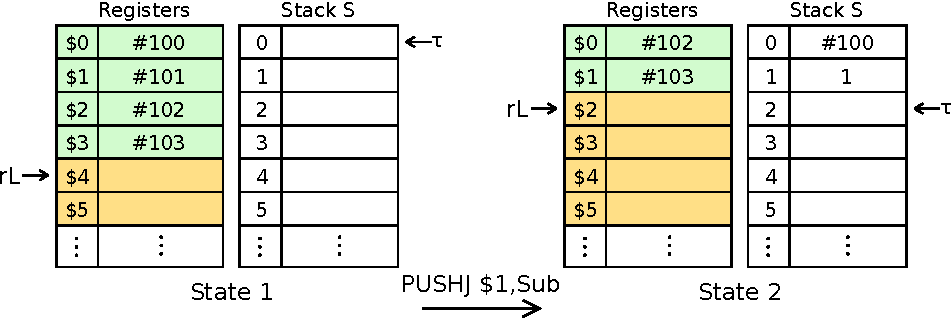
\includegraphics[width=\textwidth]{img/push-pop-user1-crop.pdf}
	\caption{Register stack: User perspective, state 1 to 2}
	\label{figure:push-pop-user1}
\end{figure}
\noindent The figure displays the used local registers green and the marginal ones orange. At first \dr{0} and \dr{1} are saved on the stack, whereas \dr{1} has been set to the number of pushed down values. Afterwards \dr{2} and \dr{3} are pushed as arguments to \i{Sub}, appearing as \dr{0} and \dr{1}. Thus, \sr{L} is 2 and $\tau$ is 2 as well.

In the next step of the example \i{Sub} performs some calculations, leading to state 3, and executes a \mi{POP 4,0} to return to the caller, whose state is shown on the right:
\begin{figure}[H]
	\centering
	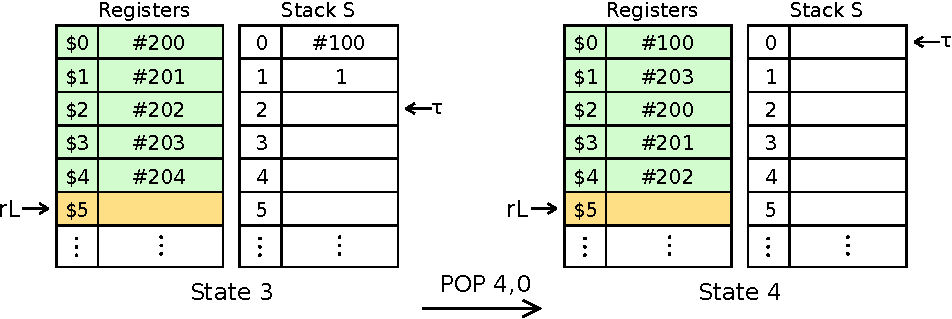
\includegraphics[width=\textwidth]{img/push-pop-user2-crop.pdf}
	\caption{Register stack: User perspective, state 3 to 4}
	\label{figure:push-pop-user2}
\end{figure}
\noindent As the figure shows, \dr{0}, \dots, \dr{4} have been set to some arbitrary values. The subsequent \mi{POP 4,0} at first loads the number of pushed down registers from the stack, \ie $S[\tau - 1] = 1$. Based on that, it restores \haddr{100} from $S[0]$ into \dr{0}, sets the hole (\dr{1}) to the last return value \haddr{203} and \dr{2}, \dots, \dr{4} to the other return values in the original order. Thus, \sr{L} is $1+{\tt X} = 5$ and $\tau$ is zero again.

At this point it might look strange that the last return value appears first for the caller, followed by the other ones in the same order they were in the registers of \i{Sub}. The section about the internal view will show the reason for that behaviour.

\paragraph{Special Cases}

Unfortunatly it is even more complicated as just described, because some special cases have been suppressed. The instructions \mi{PUSHJ|PUSHGO \$X,\dots} have the following special cases:
\begin{itemize}
	\item If $\sr{L} \le {\tt X} < \sr{G}$, the value of \sr{L} will be increased to ${\tt X} + 1$ first.
	\item If ${\tt X} \ge \sr{G}$, all local registers \dr{0}, \dots, \dr{(\sr{L} - 1)} will be saved, followed by \sr{L} and \sr{L} will be reset to zero.
\end{itemize}
On the other hand, \mi{POP X,YZ} has to take care of:
\begin{itemize}
	\item If ${\tt X} > \sr{L}$, {\tt X} will be replaced by $\sr{L} + 1$ first and the hole will be set to zero.
	\item If ${\tt X} = 0$, the hole will disappear, \ie it will become marginal.
\end{itemize}
\citep[pg. 22,23]{mmix-doc}

\subsubsection{Internal View}

After having described the procedure of calling subroutines and returning from them from the perspective of the programmer, it should be explained how MMIX does actually achieve that.

As mentioned previously, MMIX has a local register array $l$ with either 256, 512 or 1024 slots. It is used as a ring, which means that if we have the local registers $l[0]$, $l[1]$, \dots, $l[255]$, register $l[256]$ will be the same as $l[0]$, $l[257]$ the same as $l[1]$ and so on.

To realize the register stack, MMIX has to manage the registers and the stack in memory. To do so, the register ring is divided into three parts by $\alpha$, $\beta$ and $\gamma$. $l[\alpha]$, $l[\alpha+1]$, \dots, $l[\beta-1]$ are corresponding to \dr{0}, \dr{1}, \dots, \dr{(rL - 1)}. The registers $l[\beta]$, \dots, $l[\gamma-1]$ are currently unused and $l[\gamma]$, \dots, $l[\alpha-1]$ are the registers that are currently not accessible, called \i{hidden}, but have not yet been stored to memory. The situation on the stack in memory is described by the special registers \sr{O} and \sr{S}. The former is the offset of \dr{0} in memory, \ie the location it would be written to. The latter is the location the next register is going to be written to. $\alpha$, $\beta$ and $\gamma$ relate to \sr{O} and \sr{S} in the following way (when $2^n$ is the number of slots in $l$):
$$\rm\alpha=(rO/8)\bmod2^n,\qquad \beta=(\alpha+rL)\bmod2^n,\qquad
\hbox{and}\qquad \gamma=(rS/8)\bmod2^n$$

To make sure that no value is lost, MMIX has to take care that $\alpha$, $\beta$ and $\gamma$ never move past each other. Whenever a \mi{PUSHJ|PUSHGO} is done, $\alpha$ moves towards $\beta$. Setting \dr{X} with ${\tt X} \ge \sr{L}$ means that \sr{L} is increased, \ie $\beta$ is moved towards $\gamma$. If $\beta$ moved past $\gamma$, registers would have to be written to memory first to free as many slots as required. To do so, $l[\gamma]$ is written to \vmem{8}{\sr{S}} and $\gamma$ is increased by one and thus \sr{S} by 8, until the new $\beta$ is less than $\gamma$. When doing a \mi{POP}, $\alpha$ moves backwards to $\gamma$. If this moved $\alpha$ past $\gamma$, we would have to load values back from memory first. That means, $\gamma$ and \sr{S} are decreased and \vmem{8}{\sr{S}} is put into $l[\gamma]$ until the new $\alpha$ is less than $\gamma$. \citep[pg. 33]{mmix-doc}

The following figures illustrate the actions with a similar example as in the previous section. For simplicity it is assumed that only 4 local registers are present\footnote{This is not specification conform, as explained previously, but simplifies the example.}:
\begin{figure}[H]
	\centering
	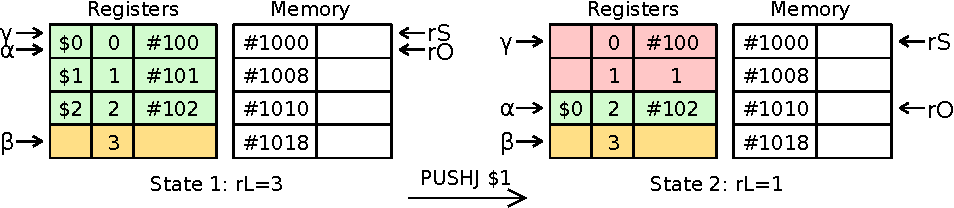
\includegraphics[width=\textwidth]{img/push-pop-internal1-crop.pdf}
	\caption{Register stack: Internal perspective, state 1 to 2}
	\label{figure:push-pop-internal1}
\end{figure}
\noindent The green and yellow cells have the same meaning as in figures \ref{figure:push-pop-user1} and \ref{figure:push-pop-user2}, while the red cells are the hidden registers. The register block on the left shows the current assignment of dynamic registers, the local register index and the value in the register. The right block displays the stack in memory with the address and the value. Additionally the values of $\alpha$, $\beta$, $\gamma$, \sr{O} and \sr{S} are indicated by pointing to the corresponding register or memory slot.

In the first state, three registers are used, $\alpha$ and $\gamma$ are zero, $\beta$ is $\alpha+\sr{L} = 3$ and \sr{O} and \sr{S} have the value \haddr{1000}. State 2 is reached by doing a \mi{PUSHJ \$1}. Hence, the offset $\alpha$ in the register ring is increased by 2 and the offset \sr{O} in memory is increased by 16. Additionally, the hole ($l[1]$) is set to the number of registers that have been pushed down.

\begin{figure}[H]
	\centering
	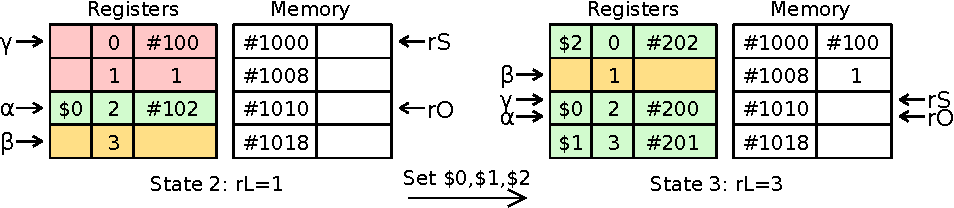
\includegraphics[width=\textwidth]{img/push-pop-internal2-crop.pdf}
	\caption{Register stack: Internal perspective, state 2 to 3}
	\label{figure:push-pop-internal2}
\end{figure}
\noindent The third state, shown in figure \ref{figure:push-pop-internal2}, is reached by setting \dr{0}, \dr{1} and \dr{2} to \haddr{200}, \haddr{201} and \haddr{202}, respectively. Setting \dr{0} does not increase \sr{L}, so that only $l[2]$ is changed. The other two both increase \sr{L} by one, \ie move $\beta$ towards $\gamma$. Thus, in each case $\gamma$ and \sr{S} are increased and a value is written to memory.

\begin{figure}[H]
	\centering
	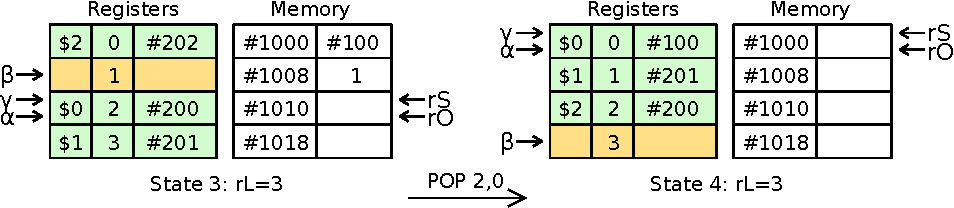
\includegraphics[width=\textwidth]{img/push-pop-internal3-crop.pdf}
	\caption{Register stack: Internal perspective, state 3 to 4}
	\label{figure:push-pop-internal3}
\end{figure}
\noindent The last transition, illustrated in figure \ref{figure:push-pop-internal3}, is achieved by doing a \mi{POP 2,0}. As described, \mi{POP} moves $\alpha$ back. The hole tells MMIX how many registers have been pushed down by the preceding \mi{PUSHJ} or \mi{PUSHGO}. In this case, the hole has been written to memory, so that it has to be loaded back first. Afterwards MMIX has to move $\alpha$ two steps up because one register has been saved and the hole has been created. To be able to decrease $\alpha$ and \sr{O}, one further value has to be loaded from memory. To return the two values, a move of $l[3]$ to $l[1]$ is sufficient because the other value is already in the desired slot (as all other return values would be, if there were more than two). This is the reason for the -- at a first glance -- strange order of the return values.

\subsection{Saving and Restoring the State}

Another concept, that works with the register stack as well, is the procedure of storing and restoring the state of the running program. It is intended both for the operating system and user applications. The former may use it for example to implement process switching or to save the state when handling an \glslink{Interrupt}{interrupt}. The latter can use it to implement thread switching in user space, for example.

\instrtblsix
	{\mi{SAVE \$X}}
	{$S[\tau{\tt ++}] \leftarrow \dr{0}, \dots, S[\tau{\tt ++}] \leftarrow \dr{(\sr{L} - 1)}$}
	{$S[\tau{\tt ++}] \leftarrow \sr{L}, \quad \sr{L} \leftarrow 0$}
	{$S[\tau{\tt ++}] \leftarrow g[\sr{G}], \dots, S[\tau{\tt ++}] \leftarrow g[255]$}
	{for $s \in \{\sr{B},\sr{D},\sr{E},\sr{H},\sr{J},\sr{M},\sr{R},\sr{P},\sr{W},\sr{X},\sr{Y},\sr{Z},(\sr{G} \ll 56) \lor \sr{A}\}$}
	{$\quad S[\tau{\tt ++}] \leftarrow s$}
	{$\dr{X} \leftarrow \tau$}
\noindent Put simply, \mi{SAVE} (\i{save process state}) stores all registers that might affect the computation on the stack and writes the address of the topmost octabyte on the stack into \dr{X}. In detail, it means that at first all hidden registers are written to memory (which is not listed in the effect description, because it shows it from the programmer perspective). Afterwards all used local registers are written behind them, followed by \sr{L} and \sr{L} is set to zero. In the next step, all global registers are written to memory, followed by the special registers that affect the computation, whose last value is an octabyte containing \sr{G} in the most significant byte and \sr{A} in the least significant ones. As will be described shortly, the value of \dr{X} after executing \mi{SAVE \$X} can be used for \mi{UNSAVE}. \citep[pg. 34]{mmix-doc}

\instrtblsix
	{\mi{UNSAVE \$Z}}
	{$\tau \leftarrow \dr{Z}$}
	{for $s \in \{(\sr{G} \ll 56) \lor \sr{A},\sr{Z},\sr{Y},\sr{X},\sr{W},\sr{P},\sr{R},\sr{M},\sr{J},\sr{H},\sr{E},\sr{D},\sr{B}\}$}
	{$\quad s \leftarrow S[{\tt --}\tau]$}
	{$g[255] \leftarrow S[{\tt --}\tau], \dots, g[\sr{G}] \leftarrow S[{\tt --}\tau]$}
	{$\sr{L} \leftarrow S[{\tt --}\tau]$}
	{$\dr{(\sr{L} - 1)} \leftarrow S[{\tt --}\tau], \dots, \dr{0} \leftarrow S[{\tt --}\tau]$}
\noindent Consequently, \mi{UNSAVE} (\i{restore process state}) goes the other way. It first sets the stack pointer to \dr{Z} and restores all special registers in the opposite order from the stack, followed by the global ones. Afterwards \sr{L} is loaded, that tells MMIX the number of local registers to restore from stack, which is done in the last step. \citep[pg. 34]{mmix-doc} It should be noted, that the hidden registers, that had been stored on the stack during \mi{SAVE} before the used local ones, are \i{not} restored by \mi{UNSAVE}. This is done by the next \mi{POP}, \ie as soon as they are needed.


\section{Interrupts and Exceptions}

As already mentioned a few times in this thesis, MMIX does of course have a concept for \glslink{Interrupt}{interrupts} and \glslink{Exception}{exceptions} as well. It distinguishes four different kinds: \i{Forced trips}, \i{dynamic trips}, \i{forced traps} and \i{dynamic traps}.\footnote{Actually, the MMIX specification speaks of three kinds, because forced trips and dynamic trips are put together. \citep[pg. 28]{mmix-doc} But taking it as a whole, forced trips and dynamic trips conceptually differ in the same way as forced traps and dynamic traps do. Therefore, this thesis speaks of four kinds.} The first two are simply called \i{trips}, while the other two are called \i{traps}. The main difference is, that trips are handled by the user application, while traps are handled by the operating system.

\subsection{Triggering of Trips and Traps}

At first, the procedure of triggering a trip or trap is described. The forced trips and traps are requested explicitly by an instruction, whereas dynamic trips and traps are either raised because an exceptional condition occurred (synchronous) or an \glslink{Interrupt}{interrupt} occurred (asynchronous).

\subsubsection{Triggering Trips}

All trips make use of the special registers \sr{B}, \sr{W}, \sr{X}, \sr{Y} and \sr{Z}. Register \sr{B} is called \i{bootstrap register} and is used to save \dr{255}. The \i{where interrupted register} \sr{W} indicates the location the interruption occurred at, \i{execution register} \sr{X} holds the 4 instruction bytes and some other information. The registers \sr{Y} and \sr{Z} (\i{Y operand} and \i{Z operand}) are used to pass operands to the trip handler. \citep[pg. 28]{mmix-doc}

A forced trip can be triggered with the following instruction:
\instrtblfive
	{\mi{TRIP X,Y,Z}}
	{$\sr{X} \leftarrow 2^{63}~|$~\vmem{4}{@}}
	{$\sr{W} \leftarrow @ + 4$}
	{$\sr{Y} \leftarrow \dr{Y},\quad \sr{Z} \leftarrow \dr{Z}$}
	{$\sr{B} \leftarrow \dr{255},\quad \dr{255} \leftarrow \sr{J}$}
	{$@ \leftarrow 0$}
\noindent As the effect description shows, \mi{TRIP} puts various information into the special registers that can be used by the handler. The {\tt X} operand of the instruction is not used by the instruction itself, but since its bytes are put into \sr{X}, the handler may utilize it. Forced trips are always handled at address 0. \citep[pg. 28]{mmix-doc} The meaning of $2^{63}$ in \sr{X} and why \sr{J} is saved, will be explained when the handling of trips and traps is described.

Dynamic trips are raised for arithmetic \glslink{Exception}{exceptions}, which are controlled by \sr{A}. The only differences to forced trips are the location they are handled at and that \sr{Y} and \sr{Z} will be set to the decoded operands of the instruction that caused the \glslink{Exception}{AE}. Each arithmetic \glslink{Exception}{exception} has its own location:
$$\vbox{\halign{\hfil#:\quad &#\hfil\cr
	\haddr{10} & Integer divide check (D)\cr
	\haddr{20} & Integer overflow (V)\cr
	\haddr{30} & Float-to-fix overflow (W)\cr
	\haddr{40} & Invalid operation (I)\cr
	\haddr{50} & Floating overflow (O)\cr
	\haddr{60} & Floating underflow (U)\cr
	\haddr{70} & Floating division by zero (Z)\cr
	\haddr{80} & Floating inexact (X)\cr
}}$$
Forced and dynamic trips are triggered in user mode only, \ie they are ignored in privileged mode. \citep[pg. 28]{mmix-doc}

\subsubsection{Triggering Traps}

Similarly to trips, traps use the special registers \sr{BB}, \sr{WW}, \sr{XX}, \sr{YY} and \sr{ZZ}, with the same purposes as their trip correspondences. The reason for the separate registers is, that a trap may of course be triggered while a trip is handled. Additionally, register \sr{T} specifies the location at which forced traps are handled, whereas \sr{TT} specifies the location for dynamic traps. \citep[pg. 28,29]{mmix-doc}

MMIX uses the special \i{interrupt mask register} \sr{K} to control which dynamic traps are enabled. As soon as a bit in the special \i{\glslink{Interrupt}{interrupt} request register} \sr{Q} is 1 and the corresponding bit in \sr{K} is 1 as well, a dynamic trap is triggered. These registers have the following layout:
\begin{figure}[H]
	\centering
	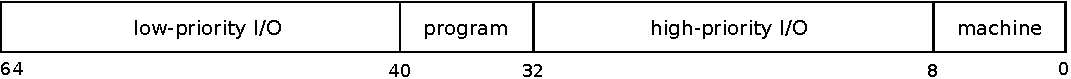
\includegraphics[width=\textwidth]{img/rKrQ-crop.pdf}
\end{figure}
\vspace{-20pt}
\noindent In general, the bits on the right have a higher priority than the bits on the left. Therefore, high-speed devices like network cards should get bits on the right, while slow devices like terminals should get bits on the left. But MMIX does not define the meanings of the I/O bits. Only the program (\glslink{Exception}{PEs}) and some of the machine bits (\glslink{Exception}{MEs}) are specified. The program bits are called {\tt rwxnkbsp} with the following meanings:
$$\vbox{\halign{{\tt #} bit: &#\hfil\cr
r	&	instruction tries to load from a page without read permission;\cr
w	&	instruction tries to store to a page without write permission;\cr
x	&	instruction appears in a page without execute permission;\cr
n	&	instruction refers to a privileged (negative) address;\cr
k	&	instruction is privileged, for use by the kernel only;\cr
b	&	instruction breaks the rules of\/ MMIX;\cr
s	&	instruction violates security (see below);\cr
p	&	instruction comes from a privileged address.\cr}}$$
The four specified machine bits from right to left stand for power failure, memory parity error, nonexistent memory and rebooting. MMIX defines, that the program bits have to be set in \sr{K} when executing in user mode (otherwise a security \glslink{Exception}{PE} is raised) and that program bit {\tt p} has to be zero in \sr{K} when executing in privileged mode (otherwise a privileged \glslink{Exception}{PE} is raised). \citep[pg. 29]{mmix-doc}

Analogous to the forced trip, the forced trap instruction is defined as:
\instrtblsix
	{\mi{TRAP X,Y,Z}}
	{$\sr{XX} \leftarrow 2^{63}~|$~\vmem{4}{@}}
	{$\sr{WW} \leftarrow @ + 4$}
	{$\sr{YY} \leftarrow \dr{Y},\quad \sr{ZZ} \leftarrow \dr{Z}$}
	{$\sr{BB} \leftarrow \dr{255},\quad \dr{255} \leftarrow \sr{J}$}
	{$\sr{K} \leftarrow 0$}
	{$@ \leftarrow \sr{T}$}
\noindent That means, besides the different handler location and the different set of special registers, \mi{TRIP} and \mi{TRAP} are equivalent, except that \mi{TRAP} clears \sr{K}. This way, dynamic traps are disabled. \citep[pg. 28]{mmix-doc} The operating system may even use instructions in a way that would raise a \glslink{Exception}{PE}, if the corresponding bit in \sr{K} were set. Because MMIX defines that "an instruction that traps with bits {\tt x}, {\tt k} or {\tt b} does nothing; a load instruction that traps with {\tt r} or {\tt n} loads zero; a store instruction that traps with any of {\tt rwxnkbsp} stores nothing" \citep[pg. 29]{mmix-doc}. The meaning of the operands {\tt X}, {\tt Y} and {\tt Z} can be defined by the operating system for any purpose. But two settings are predefined by MMIX:
\begin{enumerate}
	\item ${\tt XYZ} = 0$ should terminate the user process and
	\item ${\tt XYZ} = 1$ should offer a default action for a trip, for which the user program has not provided a handler (thus, instead of handling the trip, it can do a \mi{TRAP 0,0,1}).
\end{enumerate}

Analogous to forced and dynamic trips, the differences between forced and dynamic traps are, that for dynamic traps, the operands in \sr{YY} and \sr{ZZ} correspond to the operands of the interrupted instruction and the handler location is different. Additionally, MMIX defines that if "the interrupted instruction contributed 1s to any of the {\tt rwxnkbsp} bits of \sr{Q}, the corresponding bits are set to 1 also in \sr{XX}" \citep[pg. 29]{mmix-doc}. More precisely, these bits occur in the first byte of the upper tetra of \sr{XX}.

\subsection{Handling of Trips and Traps}

After having described the mechanisms of triggering trips and traps, it should be explained how they can be handled. This section starts with the instruction that resumes an interrupted computation, followed by the handling of trips and traps.

\subsubsection{Resuming}

Of course, MMIX has to be able to resume the ordinary execution after a trip or trap has been handled. To do so, it provides a quite sophisticated instruction that can be used for various purposes.

\instrtbleight
	{\mi{RESUME Z}}
	{if ${\tt Z} = 1$:}
	{$\quad \sr{K} \leftarrow \dr{255},\quad \dr{255} \leftarrow \sr{BB}$}
	{$@ \leftarrow \sr{W}|\sr{WW}$}
	{ropcode$~\leftarrow (\sr{X}|\sr{XX}) \gg 56$}
	{if ropcode$~= 0$: repeat(\sr{X}|\sr{XX})}
	{if ropcode$~= 1$: continue(\sr{X}|\sr{XX})}
	{if ropcode$~= 2$: set(\sr{X}|\sr{XX})}
	{if ${\tt Z} = 1~$and ropcode$~= 3$: trans(\sr{X}|\sr{XX})}
\noindent The instruction \mi{RESUME} comes in two versions: \mi{RESUME 0} resumes the computation after a trip, while \mi{RESUME 1} resumes it after a trap. Thus, \mi{RESUME 0} uses \sr{W} and \sr{X}, while \mi{RESUME 1} uses \sr{WW} and \sr{XX}. That does also mean, that the latter is prohibited in user mode. The default behaviour of \mi{RESUME}, when the so called \i{ropcode} is \haddr{80} (see \mi{TRIP} and \mi{TRAP}), is quite simple. The trip-version continues the execution at \sr{W}, while the trap-version sets \sr{K} and \dr{255} first and continues at \sr{WW} afterwards. But as the effect description shows, there are four other defined values of ropcode, which are more complicated. The four sketchy described actions have the following meaning:
\begin{itemize}
	\item repeat(\sr{X}|\sr{XX}):\\
	MMIX interprets the lower four bytes of \sr{X}|\sr{XX} as an instruction and executes it. This is allowed for all instructions except \mi{RESUME} itself.
	\item continue(\sr{X}|\sr{XX}):\\
	Continue is similar to repeat. It does also interpret the lower four bytes of \sr{X}|\sr{XX} as an instruction. But it does not use the operands provided in the instruction, but takes \sr{Y}|\sr{YY} and \sr{Z}|\sr{ZZ} instead. It is allowed for all "Set \dr{X} to the result of \dr{Y} OP \udrim{Z}" and "Set \dr{X} to the result of OP \udrim{Z}" instructions and for \mi{TRAP} as well. Some implementations of MMIX may also allow \mi{SYNCD} and \mi{SYNCID}. Another restriction is, that the instruction can not increase \sr{L}, \ie the {\tt X} operand of the instruction has to be less than \sr{L}.
	\item set(\sr{X}|\sr{XX}):\\
	This ropcode tells MMIX to set the register, denoted by the third least significant byte of \sr{X}|\sr{XX}, to \sr{Z}|\sr{ZZ}. Additionally, the third most significant byte is used to raise \glslink{Exception}{AEs}. Again, \sr{L} can not be increased.
	\item trans(\sr{X}|\sr{XX}):\\
	Last but not least, this ropcode can be used to put a translation into the translation cache. It uses \sr{YY} as the virtual address and \sr{ZZ} as the PTE and puts it into a TC. If the opcode of the instruction in the lower half of \sr{XX} is \mi{SWYM} (\i{sympathize with your machinery}; the NOP instruction of MMIX, that does nothing), the translation will be put into the instruction TC, otherwise in the data TC. Additionally, if this opcode is not \mi{SWYM}, the action repeat(\sr{XX}) will be performed.
\end{itemize}
All these actions behave as if they appeared as an instruction at location $\sr{W}|\sr{WW}-4$, \ie as if they have been inserted into the instruction stream at that position. \citep[pg. 30]{mmix-doc} It will be described shortly for what reasons the different actions, depending on ropcode, are offered.

\subsubsection{Handling Trips}

As said in the last section, all different kinds of trips have their own handler location, which are 16 bytes away from each other. That means, each handler has 4 instructions available to do what ever is necessary. For example, it could do something like:
\begin{center}
	\lstinline`PUSHJ $255,Handler; PUT rJ,$255; GET $255,rB; RESUME 0`
\end{center}
This way, the actual handler is called, saving all local registers on the stack. Before resuming, \sr{J} and \dr{255} have to be restored, because -- as described previously -- \mi{RESUME} will not do that. \citep[pg. 28]{mmix-doc}

Another way is to let the operating system perform the default actions for a trip by:
\begin{center}
	\lstinline`TRAP 0,0,1; GET $255,rB; RESUME 0`
\end{center}
In this case, no subroutine is called and thus, \sr{J} has not to be restored. \citep[pg. 28]{mmix-doc} Additionally, the reason why \mi{RESUME} does not restore the values saved by \mi{TRIP}, is that MMIX pursues the goal to perform only the minimum set of actions that are required.

When handling a dynamic trip, the operands of the instruction that caused the \glslink{Exception}{AE} are put into \sr{Y} and \sr{Z}. For example, if \mi{DIV \$0,\$1,0} is executed, MMIX will raise a division by zero \glslink{Exception}{AE} and set \sr{Y} to \$1 and \sr{Z} to 0. The handler could simply recognize that an \glslink{Exception}{AE} occurred. But it could also replace \sr{Y} and \sr{Z} with something else and change the ropcode in \sr{X} from \haddr{80} to \haddr{01} (continue). This way, the instruction would be repeated with operands \sr{Y} and \sr{Z}. Another way would be to set the ropcode to \haddr{02}, which would set \dr{X} to the value specified in \sr{Z}. \citep[pg. 28]{mmix-doc}

\subsubsection{Handling Traps}

Similarly to dynamic trips, dynamic traps that are triggered because of a \glslink{Exception}{PE}, save the operands of the instruction that caused it in \sr{YY} and \sr{ZZ}. MMIX does not define the meaning of these registers for all instructions. But it is defined that all "Set \dr{X} to the result of \dr{Y} OP \udrim{Z}" instructions put \dr{Y} in \sr{YY} and \udrim{Z} into \dr{Z}. Additionally, load instructions put the virtual address into \sr{YY}\footnote{Unfortunatly, the specification does not mention that explicitly for loads. But MMIX-PIPE does behave as explained and it would make no sense to do it for store instructions, but not for load instructions. After all, both may trigger a protection fault, for which the operating system has to know the virtual address. Having to calculate it from the {\tt Y} and {\tt Z} operand of the instruction for loads and simply read it from \sr{YY} for stores, would be very strange.}, while store instructions do additionally put the octa to be stored (including unchanged bytes for cases like \mi{STB}) into \sr{ZZ}. \citep[pg. 27]{mmix-doc}

Additionally it is noteworthy, that the OS has not many choices when considering \glslink{Exception}{PE} handling. Because the only \glslink{Exception}{PEs}, which are well defined, are the protection faults. For all others, \ie when refering to a negative address, using a privileged instruction, breaking the rules of MMIX, violating security or jumping to a privileged address, the MMIX specification does not define the values of \sr{WW} and \sr{XX}. Thus, the operating system is unable to resume the computation of the user program in a reliable way. But of course, these \glslink{Exception}{PEs} indicate a malicious or faulty user program anyway, so that the best option is a kill (and perhaps providing feedback to the user in form of a log entry or similar).

MMIX does also allow cheaper implementations of it, that let the software realize some instructions. In this case, these instructions cause a forced trap. For example, expensive operations like \mi{DIV} or \mi{FREM} could be implemented in software by checking the opcode in \sr{XX} when handling a forced trap. If it is one of these instructions, the result will be computed, put into \sr{ZZ} and the ropcode will be set to \haddr{02}. A subsequent \mi{RESUME 1} will place \sr{ZZ} into the desired register. As already said, even arithmetic \glslink{Exception}{exceptions} could be raised by specifying them in the third most significant byte of \sr{XX}. \citep[pg. 28]{mmix-doc}

A similar feature is, that address translation can be done in software. This can be requested by setting field $f$ of \sr{V} to 1, but some implementations of MMIX might even require that. As soon as a translation is necessary, \ie it is not already in the corresponding TC, a forced trap with ropcode \haddr{03} is triggered. The virtual address will be available in \sr{YY}. When the translation is done, the handler should put the physical address into \sr{ZZ}. A subsequent \mi{RESUME 1} will put this translation into the TC and repeat the instruction, which will succeed this time. It should be noted, that if an instruction fetch fails, MMIX will put the instruction \mi{SWYM} into \sr{XX}. This way, the translation will be put into the instruction TC and the fetch will be repeated when \mi{RESUME 1} is executed. \citep[pg. 28]{mmix-doc}

\subsection{Interruptibility}
\label{sec:mmix-interruptibility}

Because of the complexity of some instructions (like \mi{SAVE}, \mi{POP}, \mi{DIV}, \mi{FREM} and so on), MMIX allows them to be interruptible. The specification words it as:
\begin{quote}
Non-catastrophic \glslink{Interrupt}{interrupts} in MMIX are always precise, in the sense that all legal instructions before a certain point have effectively been executed, and no instructions after that point have yet been executed. The current instruction, which may or may not have been completed at the time of \glslink{Interrupt}{interrupt} and which may or may not need to be resumed after the \glslink{Interrupt}{interrupt} has been serviced, is put into the special execution register \sr{X}, and its operands (if any) are placed in special registers \sr{Y} and \sr{Z}.\footnote{Actually, \sr{XX}, \sr{YY} and \sr{ZZ} are meant (which were introduced later in the specification), because the other ones are only used for trips, which are either explicitly requested or raised for \glslink{Exception}{AEs}. Thus, they do not occur at arbitrary points of time during a computation, as \glslink{Interrupt}{interrupts} from I/O devices may.} \citep[pg. 27]{mmix-doc}
\end{quote}
That means, if an \glslink{Interrupt}{interrupt} occurs while executing an instruction, a particular MMIX implementation may wait briefly until an interruption is possible and then put the state of computation of the current instruction into \sr{XX}, \sr{YY} and \sr{ZZ}. In this case, the meaning of the registers is completely implementation dependent. For example, \mi{FREM \$X,\$Y,\$Z} may set \sr{YY} and \sr{ZZ}, such that $\sr{YY} \bmod \sr{ZZ} = \dr{Y} \bmod \dr{Z}$, but the actual values of \sr{YY} and \sr{ZZ} may be different than \dr{Y} and \dr{Z}. \citep[pg. 27 and 29]{mmix-doc} If MMIX sets ropcode to \haddr{01} (continue), the operating system will not be required to care about that, because a \mi{RESUME 1} will simply execute that instruction again with \sr{YY} and \sr{ZZ}, which will lead to the same result.

It should also be mentioned, that \sr{XX} might not hold the instruction found at address $\sr{WW}-4$. Not only because of jumps, but also because MMIX might put an instruction into \sr{XX}, that has been inserted internally. For example, if \mi{ADD \$X,\$Y,\$Z} is executed with ${\tt X} \ge \sr{L}$, the hardware may insert an instruction to increase \sr{L} first.



